\documentclass[twoside]{book}

% Packages required by doxygen
\usepackage{calc}
\usepackage{doxygen}
\usepackage{graphicx}
\usepackage[utf8]{inputenc}
\usepackage{makeidx}
\usepackage{multicol}
\usepackage{multirow}
\usepackage{textcomp}
\usepackage[table]{xcolor}

% Font selection
\usepackage[T1]{fontenc}
\usepackage{mathptmx}
\usepackage[scaled=.90]{helvet}
\usepackage{courier}
\usepackage{amssymb}
\usepackage{sectsty}
\renewcommand{\familydefault}{\sfdefault}
\allsectionsfont{%
  \fontseries{bc}\selectfont%
  \color{darkgray}%
}
\renewcommand{\DoxyLabelFont}{%
  \fontseries{bc}\selectfont%
  \color{darkgray}%
}

% Page & text layout
\usepackage{geometry}
\geometry{%
  a4paper,%
  top=2.5cm,%
  bottom=2.5cm,%
  left=2.5cm,%
  right=2.5cm%
}
\tolerance=750
\hfuzz=15pt
\hbadness=750
\setlength{\emergencystretch}{15pt}
\setlength{\parindent}{0cm}
\setlength{\parskip}{0.2cm}
\makeatletter
\renewcommand{\paragraph}{%
  \@startsection{paragraph}{4}{0ex}{-1.0ex}{1.0ex}{%
    \normalfont\normalsize\bfseries\SS@parafont%
  }%
}
\renewcommand{\subparagraph}{%
  \@startsection{subparagraph}{5}{0ex}{-1.0ex}{1.0ex}{%
    \normalfont\normalsize\bfseries\SS@subparafont%
  }%
}
\makeatother

% Headers & footers
\usepackage{fancyhdr}
\pagestyle{fancyplain}
\fancyhead[LE]{\fancyplain{}{\bfseries\thepage}}
\fancyhead[CE]{\fancyplain{}{}}
\fancyhead[RE]{\fancyplain{}{\bfseries\leftmark}}
\fancyhead[LO]{\fancyplain{}{\bfseries\rightmark}}
\fancyhead[CO]{\fancyplain{}{}}
\fancyhead[RO]{\fancyplain{}{\bfseries\thepage}}
\fancyfoot[LE]{\fancyplain{}{}}
\fancyfoot[CE]{\fancyplain{}{}}
\fancyfoot[RE]{\fancyplain{}{\bfseries\scriptsize Generated on Mon Nov 25 2013 18:48:10 for Swird / Swrid by Doxygen }}
\fancyfoot[LO]{\fancyplain{}{\bfseries\scriptsize Generated on Mon Nov 25 2013 18:48:10 for Swird / Swrid by Doxygen }}
\fancyfoot[CO]{\fancyplain{}{}}
\fancyfoot[RO]{\fancyplain{}{}}
\renewcommand{\footrulewidth}{0.4pt}
\renewcommand{\chaptermark}[1]{%
  \markboth{#1}{}%
}
\renewcommand{\sectionmark}[1]{%
  \markright{\thesection\ #1}%
}

% Indices & bibliography
\usepackage{natbib}
\usepackage[titles]{tocloft}
\setcounter{tocdepth}{3}
\setcounter{secnumdepth}{5}
\makeindex

% Hyperlinks (required, but should be loaded last)
\usepackage{ifpdf}
\ifpdf
  \usepackage[pdftex,pagebackref=true]{hyperref}
\else
  \usepackage[ps2pdf,pagebackref=true]{hyperref}
\fi
\hypersetup{%
  colorlinks=true,%
  linkcolor=blue,%
  citecolor=blue,%
  unicode%
}

% Custom commands
\newcommand{\clearemptydoublepage}{%
  \newpage{\pagestyle{empty}\cleardoublepage}%
}


%===== C O N T E N T S =====

\begin{document}

% Titlepage & ToC
\hypersetup{pageanchor=false}
\pagenumbering{roman}
\begin{titlepage}
\vspace*{7cm}
\begin{center}%
{\Large Swird / Swrid }\\
\vspace*{1cm}
{\large Generated by Doxygen 1.8.4}\\
\vspace*{0.5cm}
{\small Mon Nov 25 2013 18:48:10}\\
\end{center}
\end{titlepage}
\clearemptydoublepage
\tableofcontents
\clearemptydoublepage
\pagenumbering{arabic}
\hypersetup{pageanchor=true}

%--- Begin generated contents ---
\chapter{Hierarchical Index}
\section{\-Class \-Hierarchy}
\-This inheritance list is sorted roughly, but not completely, alphabetically\-:\begin{DoxyCompactList}
\item \contentsline{section}{\-Button}{\pageref{class_button}}{}
\item \contentsline{section}{\-Element}{\pageref{class_element}}{}
\begin{DoxyCompactList}
\item \contentsline{section}{\-Base\-Element}{\pageref{class_base_element}}{}
\begin{DoxyCompactList}
\item \contentsline{section}{\-Point\-Bonus\-Element}{\pageref{class_point_bonus_element}}{}
\end{DoxyCompactList}
\end{DoxyCompactList}
\item \contentsline{section}{\-Element\-U\-I}{\pageref{class_element_u_i}}{}
\item \contentsline{section}{\-Engine}{\pageref{class_engine}}{}
\item \contentsline{section}{\-Grid}{\pageref{class_grid}}{}
\item \contentsline{section}{\-Grid\-Mode}{\pageref{class_grid_mode}}{}
\begin{DoxyCompactList}
\item \contentsline{section}{\-Grid\-Mode\-Hard}{\pageref{class_grid_mode_hard}}{}
\item \contentsline{section}{\-Grid\-Mode\-Normal}{\pageref{class_grid_mode_normal}}{}
\end{DoxyCompactList}
\item \contentsline{section}{\-Player}{\pageref{class_player}}{}
\item \contentsline{section}{\-Screen}{\pageref{class_screen}}{}
\begin{DoxyCompactList}
\item \contentsline{section}{\-Game\-Screen}{\pageref{class_game_screen}}{}
\item \contentsline{section}{\-Menu\-Screen}{\pageref{class_menu_screen}}{}
\end{DoxyCompactList}
\end{DoxyCompactList}

\chapter{Class Index}
\section{Class List}
Here are the classes, structs, unions and interfaces with brief descriptions\-:\begin{DoxyCompactList}
\item\contentsline{section}{\hyperlink{classBaseElement}{Base\-Element} \\*Décorateur de la classe \hyperlink{classElement}{Element} }{\pageref{classBaseElement}}{}
\item\contentsline{section}{\hyperlink{classButton}{Button} \\*La classe de gestion des boutons }{\pageref{classButton}}{}
\item\contentsline{section}{\hyperlink{classElement}{Element} \\*La classe de gestion des éléments }{\pageref{classElement}}{}
\item\contentsline{section}{\hyperlink{classElementUI}{Element\-U\-I} \\*Classe gérant l'affichage graphique des éléments }{\pageref{classElementUI}}{}
\item\contentsline{section}{\hyperlink{classEngine}{Engine} \\*La classe \hyperlink{classEngine}{Engine}, moteur du jeu }{\pageref{classEngine}}{}
\item\contentsline{section}{\hyperlink{classGameScreen}{Game\-Screen} \\*La classe \hyperlink{classGameScreen}{Game\-Screen}, gestion de l'écran de jeu implémente l'interface \hyperlink{classScreen}{Screen} }{\pageref{classGameScreen}}{}
\item\contentsline{section}{\hyperlink{classGrid}{Grid} \\*La classe \hyperlink{classGrid}{Grid}, classe de gestion de la grille de jeu }{\pageref{classGrid}}{}
\item\contentsline{section}{\hyperlink{classGridMode}{Grid\-Mode} \\*Interface \hyperlink{classGridMode}{Grid\-Mode} }{\pageref{classGridMode}}{}
\item\contentsline{section}{\hyperlink{classGridModeHard}{Grid\-Mode\-Hard} \\*La classe \hyperlink{classGridModeHard}{Grid\-Mode\-Hard}, implémente la \hyperlink{classGridMode}{Grid\-Mode} }{\pageref{classGridModeHard}}{}
\item\contentsline{section}{\hyperlink{classGridModeNormal}{Grid\-Mode\-Normal} \\*La classe \hyperlink{classGridModeNormal}{Grid\-Mode\-Normal}, implémente la \hyperlink{classGridMode}{Grid\-Mode} }{\pageref{classGridModeNormal}}{}
\item\contentsline{section}{\hyperlink{classMenuScreen}{Menu\-Screen} \\*La classe \hyperlink{classMenuScreen}{Menu\-Screen}, Implémente l'interface \hyperlink{classScreen}{Screen} }{\pageref{classMenuScreen}}{}
\item\contentsline{section}{\hyperlink{classPlayer}{Player} \\*La classe \hyperlink{classPlayer}{Player} }{\pageref{classPlayer}}{}
\item\contentsline{section}{\hyperlink{classPointBonusElement}{Point\-Bonus\-Element} \\*La classe \hyperlink{classPointBonusElement}{Point\-Bonus\-Element}, hérite de \hyperlink{classBaseElement}{Base\-Element} }{\pageref{classPointBonusElement}}{}
\item\contentsline{section}{\hyperlink{classScreen}{Screen} \\*Interface \hyperlink{classScreen}{Screen} }{\pageref{classScreen}}{}
\end{DoxyCompactList}

\chapter{Class Documentation}
\hypertarget{classBaseElement}{\section{Base\-Element Class Reference}
\label{classBaseElement}\index{Base\-Element@{Base\-Element}}
}


Décorateur de la classe \hyperlink{classElement}{Element}.  




{\ttfamily \#include $<$Base\-Element.\-h$>$}

Inheritance diagram for Base\-Element\-:\begin{figure}[H]
\begin{center}
\leavevmode
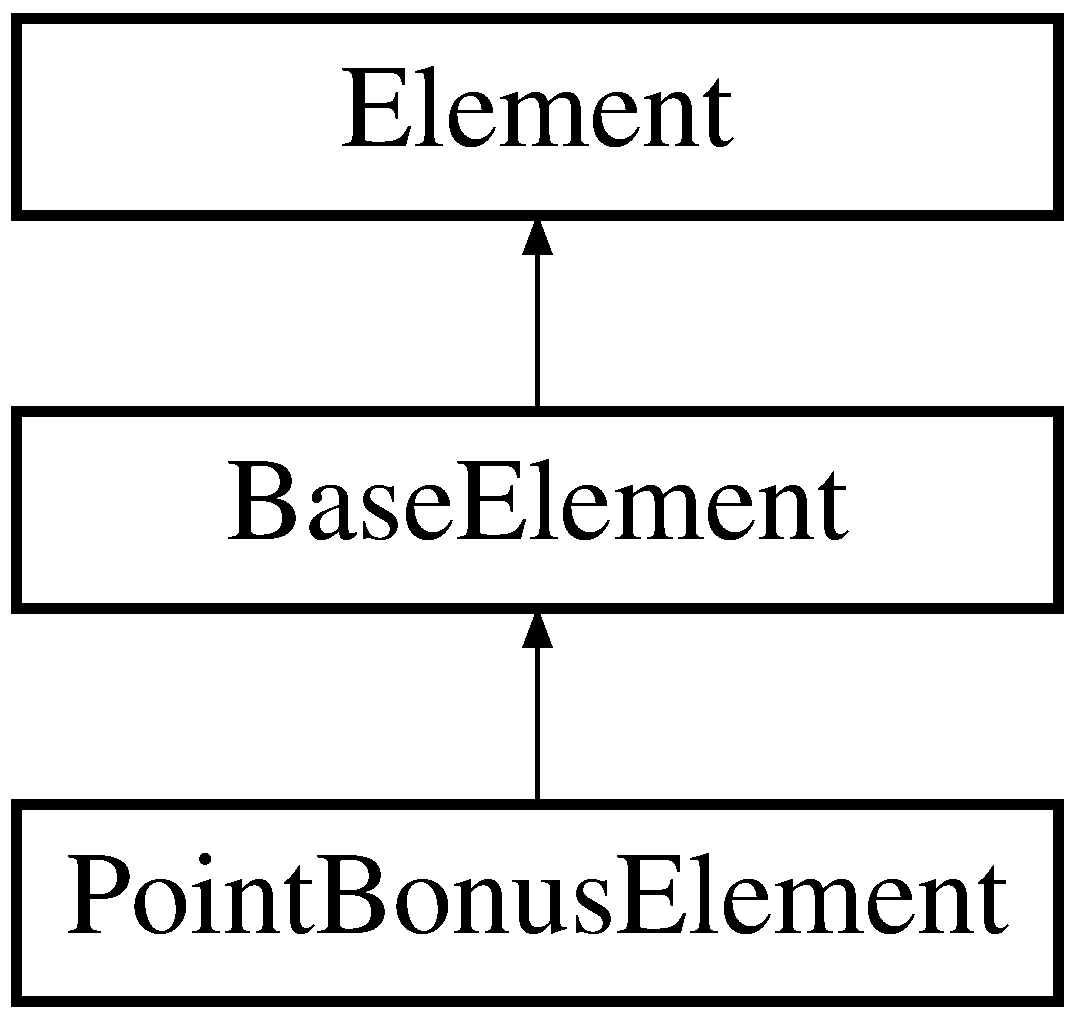
\includegraphics[height=3.000000cm]{classBaseElement}
\end{center}
\end{figure}
\subsection*{Public Member Functions}
\begin{DoxyCompactItemize}
\item 
\hyperlink{classBaseElement_a1569ee70076588b3b6d28e4e17257de0}{Base\-Element} ()
\begin{DoxyCompactList}\small\item\em Constructeur. \end{DoxyCompactList}\item 
\hyperlink{classBaseElement_a4b5096047820c9447786bad867495eec}{Base\-Element} (\hyperlink{classElement}{Element} el)
\begin{DoxyCompactList}\small\item\em surchage du constructeur \end{DoxyCompactList}\item 
virtual \hyperlink{classBaseElement_ad670a437f6c567beb80294850de2ff13}{$\sim$\-Base\-Element} ()
\begin{DoxyCompactList}\small\item\em Destructeur. \end{DoxyCompactList}\item 
int \hyperlink{classBaseElement_a7ffb8e8f1cf88ae0a8489d8e653301a2}{get\-Value} ()
\begin{DoxyCompactList}\small\item\em Accesseur de l'attribut value. \end{DoxyCompactList}\item 
int \hyperlink{classBaseElement_ad1b8117c4a21129c759bbee82e024347}{get\-Money} ()
\begin{DoxyCompactList}\small\item\em Accesseur de l'attribut money. \end{DoxyCompactList}\item 
int \hyperlink{classBaseElement_a419e6be2effe678ce8d762d267f24840}{get\-Type} ()
\begin{DoxyCompactList}\small\item\em Accesseur de l'attribut type. \end{DoxyCompactList}\item 
void \hyperlink{classBaseElement_aa05ade655a8c57b870971fdcc5ae45e4}{set\-Type} (int type)
\begin{DoxyCompactList}\small\item\em setteur de l'attribut value \end{DoxyCompactList}\end{DoxyCompactItemize}
\subsection*{Protected Attributes}
\begin{DoxyCompactItemize}
\item 
\hypertarget{classBaseElement_a55731b2b461cc786987edbf2e0236b7e}{\hyperlink{classElement}{Element} \hyperlink{classBaseElement_a55731b2b461cc786987edbf2e0236b7e}{el\-\_\-}}\label{classBaseElement_a55731b2b461cc786987edbf2e0236b7e}

\begin{DoxyCompactList}\small\item\em L'attribut de type \hyperlink{classElement}{Element}. \end{DoxyCompactList}\item 
\hypertarget{classBaseElement_a2e495347f94ec3a9d6622b9e69649f58}{int \hyperlink{classBaseElement_a2e495347f94ec3a9d6622b9e69649f58}{bonus\-Value\-\_\-}}\label{classBaseElement_a2e495347f94ec3a9d6622b9e69649f58}

\begin{DoxyCompactList}\small\item\em L'attribut valeur du bonus de type entier. \end{DoxyCompactList}\item 
\hypertarget{classBaseElement_a61a308a2b91324b62ee50a3aa1235dbe}{int \hyperlink{classBaseElement_a61a308a2b91324b62ee50a3aa1235dbe}{bonus\-Money\-\_\-}}\label{classBaseElement_a61a308a2b91324b62ee50a3aa1235dbe}

\begin{DoxyCompactList}\small\item\em L'attribut bonus. \end{DoxyCompactList}\end{DoxyCompactItemize}


\subsection{Detailed Description}
Décorateur de la classe \hyperlink{classElement}{Element}. 

Ajout (ou non) d'un bonus sur les éléments 

\subsection{Constructor \& Destructor Documentation}
\hypertarget{classBaseElement_a1569ee70076588b3b6d28e4e17257de0}{\index{Base\-Element@{Base\-Element}!Base\-Element@{Base\-Element}}
\index{Base\-Element@{Base\-Element}!BaseElement@{Base\-Element}}
\subsubsection[{Base\-Element}]{\setlength{\rightskip}{0pt plus 5cm}Base\-Element\-::\-Base\-Element (
\begin{DoxyParamCaption}
{}
\end{DoxyParamCaption}
)}}\label{classBaseElement_a1569ee70076588b3b6d28e4e17257de0}


Constructeur. 

Constructeur de la classe \hyperlink{classBaseElement}{Base\-Element} \hypertarget{classBaseElement_a4b5096047820c9447786bad867495eec}{\index{Base\-Element@{Base\-Element}!Base\-Element@{Base\-Element}}
\index{Base\-Element@{Base\-Element}!BaseElement@{Base\-Element}}
\subsubsection[{Base\-Element}]{\setlength{\rightskip}{0pt plus 5cm}Base\-Element\-::\-Base\-Element (
\begin{DoxyParamCaption}
\item[{{\bf Element}}]{el}
\end{DoxyParamCaption}
)}}\label{classBaseElement_a4b5096047820c9447786bad867495eec}


surchage du constructeur 

Surcharge du constructeur de la classe \hyperlink{classBaseElement}{Base\-Element}


\begin{DoxyParams}{Parameters}
{\em \hyperlink{classElement}{Element}} & \-: L'élément à décorer \\
\hline
\end{DoxyParams}
\hypertarget{classBaseElement_ad670a437f6c567beb80294850de2ff13}{\index{Base\-Element@{Base\-Element}!$\sim$\-Base\-Element@{$\sim$\-Base\-Element}}
\index{$\sim$\-Base\-Element@{$\sim$\-Base\-Element}!BaseElement@{Base\-Element}}
\subsubsection[{$\sim$\-Base\-Element}]{\setlength{\rightskip}{0pt plus 5cm}virtual Base\-Element\-::$\sim$\-Base\-Element (
\begin{DoxyParamCaption}
{}
\end{DoxyParamCaption}
)\hspace{0.3cm}{\ttfamily [virtual]}}}\label{classBaseElement_ad670a437f6c567beb80294850de2ff13}


Destructeur. 

Destructeur de la classe \hyperlink{classBaseElement}{Base\-Element} 

\subsection{Member Function Documentation}
\hypertarget{classBaseElement_ad1b8117c4a21129c759bbee82e024347}{\index{Base\-Element@{Base\-Element}!get\-Money@{get\-Money}}
\index{get\-Money@{get\-Money}!BaseElement@{Base\-Element}}
\subsubsection[{get\-Money}]{\setlength{\rightskip}{0pt plus 5cm}int Base\-Element\-::get\-Money (
\begin{DoxyParamCaption}
{}
\end{DoxyParamCaption}
)}}\label{classBaseElement_ad1b8117c4a21129c759bbee82e024347}


Accesseur de l'attribut money. 

Méthode qui retourne la valeur de l'attribut money \begin{DoxyReturn}{Returns}
entier ; 
\end{DoxyReturn}
\hypertarget{classBaseElement_a419e6be2effe678ce8d762d267f24840}{\index{Base\-Element@{Base\-Element}!get\-Type@{get\-Type}}
\index{get\-Type@{get\-Type}!BaseElement@{Base\-Element}}
\subsubsection[{get\-Type}]{\setlength{\rightskip}{0pt plus 5cm}int Base\-Element\-::get\-Type (
\begin{DoxyParamCaption}
{}
\end{DoxyParamCaption}
)}}\label{classBaseElement_a419e6be2effe678ce8d762d267f24840}


Accesseur de l'attribut type. 

Méthode qui retourne la valeur de l'attribut type \begin{DoxyReturn}{Returns}
entier ; 
\end{DoxyReturn}
\hypertarget{classBaseElement_a7ffb8e8f1cf88ae0a8489d8e653301a2}{\index{Base\-Element@{Base\-Element}!get\-Value@{get\-Value}}
\index{get\-Value@{get\-Value}!BaseElement@{Base\-Element}}
\subsubsection[{get\-Value}]{\setlength{\rightskip}{0pt plus 5cm}int Base\-Element\-::get\-Value (
\begin{DoxyParamCaption}
{}
\end{DoxyParamCaption}
)}}\label{classBaseElement_a7ffb8e8f1cf88ae0a8489d8e653301a2}


Accesseur de l'attribut value. 

Méthode qui retourne la valeur de l'attribut value \begin{DoxyReturn}{Returns}
entier ; 
\end{DoxyReturn}
\hypertarget{classBaseElement_aa05ade655a8c57b870971fdcc5ae45e4}{\index{Base\-Element@{Base\-Element}!set\-Type@{set\-Type}}
\index{set\-Type@{set\-Type}!BaseElement@{Base\-Element}}
\subsubsection[{set\-Type}]{\setlength{\rightskip}{0pt plus 5cm}void Base\-Element\-::set\-Type (
\begin{DoxyParamCaption}
\item[{int}]{type}
\end{DoxyParamCaption}
)}}\label{classBaseElement_aa05ade655a8c57b870971fdcc5ae45e4}


setteur de l'attribut value 

Méthode qui retourne la valeur de l'attribut value \begin{DoxyReturn}{Returns}
entier ; 
\end{DoxyReturn}


The documentation for this class was generated from the following file\-:\begin{DoxyCompactItemize}
\item 
include/Base\-Element.\-h\end{DoxyCompactItemize}

\hypertarget{classButton}{\section{Button Class Reference}
\label{classButton}\index{Button@{Button}}
}


La classe de gestion des boutons.  




{\ttfamily \#include $<$Button.\-h$>$}

\subsection*{Public Member Functions}
\begin{DoxyCompactItemize}
\item 
\hyperlink{classButton_a6e5fe59a2412635f037cdacdec3ffbf4}{Button} (int x, int y)
\begin{DoxyCompactList}\small\item\em Constructeur. \end{DoxyCompactList}\item 
virtual \hyperlink{classButton_a6d35cf666b119be6153a717427f9b5e2}{$\sim$\-Button} ()
\begin{DoxyCompactList}\small\item\em Destructeur. \end{DoxyCompactList}\item 
S\-D\-L\-\_\-\-Rect \hyperlink{classButton_ad1c08a85ce4226d52407bedac09faad4}{Getbutton\-Position} ()
\begin{DoxyCompactList}\small\item\em Accesseur de l'attribut button\-Position. \end{DoxyCompactList}\item 
void \hyperlink{classButton_ad0ebac62e6517157d7064798a0a6f79b}{Setbutton\-Position} (S\-D\-L\-\_\-\-Rect val)
\begin{DoxyCompactList}\small\item\em setteur de l'attribut Button\-Position \end{DoxyCompactList}\item 
void \hyperlink{classButton_ad8af591aa138c802d1708e772fab38e1}{apply\-Button} (S\-D\-L\-\_\-\-Surface $\ast$surface)
\begin{DoxyCompactList}\small\item\em mise en place du bouton sur une surface \end{DoxyCompactList}\item 
bool \hyperlink{classButton_a2a29ddfaae95ff59d44815c5a896d57b}{check\-Click} (int mouse\-X, int mouse\-Y)
\begin{DoxyCompactList}\small\item\em vérification du clique sur le bouton \end{DoxyCompactList}\item 
void \hyperlink{classButton_adcc14081549c1c21b6ac58df70a4dbdb}{set\-State} (int state)
\begin{DoxyCompactList}\small\item\em changement d'état du bouton \end{DoxyCompactList}\item 
void \hyperlink{classButton_ab31b0993b959cf9863eb2cf22a7ae18b}{free} ()
\begin{DoxyCompactList}\small\item\em Libération de la mémoire. \end{DoxyCompactList}\item 
void \hyperlink{classButton_a37a5a9964f62a28929e63b9d2e067c5a}{init} (const char $\ast$path1, const char $\ast$path2)
\begin{DoxyCompactList}\small\item\em Initialisation du bouton. \end{DoxyCompactList}\end{DoxyCompactItemize}


\subsection{Detailed Description}
La classe de gestion des boutons. 

\subsection{Constructor \& Destructor Documentation}
\hypertarget{classButton_a6e5fe59a2412635f037cdacdec3ffbf4}{\index{Button@{Button}!Button@{Button}}
\index{Button@{Button}!Button@{Button}}
\subsubsection[{Button}]{\setlength{\rightskip}{0pt plus 5cm}Button\-::\-Button (
\begin{DoxyParamCaption}
\item[{int}]{x, }
\item[{int}]{y}
\end{DoxyParamCaption}
)}}\label{classButton_a6e5fe59a2412635f037cdacdec3ffbf4}


Constructeur. 

Constructeur de la classe \hyperlink{classButton}{Button} \hypertarget{classButton_a6d35cf666b119be6153a717427f9b5e2}{\index{Button@{Button}!$\sim$\-Button@{$\sim$\-Button}}
\index{$\sim$\-Button@{$\sim$\-Button}!Button@{Button}}
\subsubsection[{$\sim$\-Button}]{\setlength{\rightskip}{0pt plus 5cm}virtual Button\-::$\sim$\-Button (
\begin{DoxyParamCaption}
{}
\end{DoxyParamCaption}
)\hspace{0.3cm}{\ttfamily [virtual]}}}\label{classButton_a6d35cf666b119be6153a717427f9b5e2}


Destructeur. 

Destructeur de la classe \hyperlink{classButton}{Button} 

\subsection{Member Function Documentation}
\hypertarget{classButton_ad8af591aa138c802d1708e772fab38e1}{\index{Button@{Button}!apply\-Button@{apply\-Button}}
\index{apply\-Button@{apply\-Button}!Button@{Button}}
\subsubsection[{apply\-Button}]{\setlength{\rightskip}{0pt plus 5cm}void Button\-::apply\-Button (
\begin{DoxyParamCaption}
\item[{S\-D\-L\-\_\-\-Surface $\ast$}]{surface}
\end{DoxyParamCaption}
)}}\label{classButton_ad8af591aa138c802d1708e772fab38e1}


mise en place du bouton sur une surface 

Méthode qui permet de mettre en place le bouton sur une surface 
\begin{DoxyParams}{Parameters}
{\em S\-D\-L\-\_\-surface} & la surface sur laquelle on \char`\"{}place\char`\"{} l'image \\
\hline
\end{DoxyParams}
\hypertarget{classButton_a2a29ddfaae95ff59d44815c5a896d57b}{\index{Button@{Button}!check\-Click@{check\-Click}}
\index{check\-Click@{check\-Click}!Button@{Button}}
\subsubsection[{check\-Click}]{\setlength{\rightskip}{0pt plus 5cm}bool Button\-::check\-Click (
\begin{DoxyParamCaption}
\item[{int}]{mouse\-X, }
\item[{int}]{mouse\-Y}
\end{DoxyParamCaption}
)}}\label{classButton_a2a29ddfaae95ff59d44815c5a896d57b}


vérification du clique sur le bouton 

Méthode qui permet de s'assurer qu'on clique sur le bouton 
\begin{DoxyParams}{Parameters}
{\em entier} & mouse\-X l'abscisse du clique sur l'écran \\
\hline
{\em entier} & mousey l'ordonnée du clique sur l'écran \\
\hline
\end{DoxyParams}
\begin{DoxyReturn}{Returns}
booléen true si le clique est bien sur le bouton,false sinon 
\end{DoxyReturn}
\hypertarget{classButton_ab31b0993b959cf9863eb2cf22a7ae18b}{\index{Button@{Button}!free@{free}}
\index{free@{free}!Button@{Button}}
\subsubsection[{free}]{\setlength{\rightskip}{0pt plus 5cm}void Button\-::free (
\begin{DoxyParamCaption}
{}
\end{DoxyParamCaption}
)}}\label{classButton_ab31b0993b959cf9863eb2cf22a7ae18b}


Libération de la mémoire. 

Méthode qui permet de la mémoire liée aux surfaces utilisées pour le bouton \hypertarget{classButton_ad1c08a85ce4226d52407bedac09faad4}{\index{Button@{Button}!Getbutton\-Position@{Getbutton\-Position}}
\index{Getbutton\-Position@{Getbutton\-Position}!Button@{Button}}
\subsubsection[{Getbutton\-Position}]{\setlength{\rightskip}{0pt plus 5cm}S\-D\-L\-\_\-\-Rect Button\-::\-Getbutton\-Position (
\begin{DoxyParamCaption}
{}
\end{DoxyParamCaption}
)\hspace{0.3cm}{\ttfamily [inline]}}}\label{classButton_ad1c08a85ce4226d52407bedac09faad4}


Accesseur de l'attribut button\-Position. 

Méthode qui retourne la S\-D\-L\-\_\-\-Rec du boutton \begin{DoxyReturn}{Returns}
S\-D\-L\-\_\-\-Rec ; 
\end{DoxyReturn}
\hypertarget{classButton_a37a5a9964f62a28929e63b9d2e067c5a}{\index{Button@{Button}!init@{init}}
\index{init@{init}!Button@{Button}}
\subsubsection[{init}]{\setlength{\rightskip}{0pt plus 5cm}void Button\-::init (
\begin{DoxyParamCaption}
\item[{const char $\ast$}]{path1, }
\item[{const char $\ast$}]{path2}
\end{DoxyParamCaption}
)}}\label{classButton_a37a5a9964f62a28929e63b9d2e067c5a}


Initialisation du bouton. 

Méthode qui permet d'initialiser le bouton avec le chemin d'accès au images correspondante 
\begin{DoxyParams}{Parameters}
{\em const} & char$\ast$ , le chemin d'accès à la première image \\
\hline
{\em const} & char$\ast$, le chemin d'accès à la deuxième image \\
\hline
\end{DoxyParams}
\hypertarget{classButton_ad0ebac62e6517157d7064798a0a6f79b}{\index{Button@{Button}!Setbutton\-Position@{Setbutton\-Position}}
\index{Setbutton\-Position@{Setbutton\-Position}!Button@{Button}}
\subsubsection[{Setbutton\-Position}]{\setlength{\rightskip}{0pt plus 5cm}void Button\-::\-Setbutton\-Position (
\begin{DoxyParamCaption}
\item[{S\-D\-L\-\_\-\-Rect}]{val}
\end{DoxyParamCaption}
)\hspace{0.3cm}{\ttfamily [inline]}}}\label{classButton_ad0ebac62e6517157d7064798a0a6f79b}


setteur de l'attribut Button\-Position 

Méthode qui affecte une valeur à l'attribut button\-Position 
\begin{DoxyParams}{Parameters}
{\em S\-D\-L\-\_\-\-Rec} & \-: une nouvelle S\-D\-L\-\_\-\-Rec \\
\hline
\end{DoxyParams}
\hypertarget{classButton_adcc14081549c1c21b6ac58df70a4dbdb}{\index{Button@{Button}!set\-State@{set\-State}}
\index{set\-State@{set\-State}!Button@{Button}}
\subsubsection[{set\-State}]{\setlength{\rightskip}{0pt plus 5cm}void Button\-::set\-State (
\begin{DoxyParamCaption}
\item[{int}]{state}
\end{DoxyParamCaption}
)}}\label{classButton_adcc14081549c1c21b6ac58df70a4dbdb}


changement d'état du bouton 

Méthode qui permet de changer l'état du bouton 
\begin{DoxyParams}{Parameters}
{\em entier} & correspondant a un état \\
\hline
\end{DoxyParams}


The documentation for this class was generated from the following file\-:\begin{DoxyCompactItemize}
\item 
include/Button.\-h\end{DoxyCompactItemize}

\hypertarget{classElement}{\section{Element Class Reference}
\label{classElement}\index{Element@{Element}}
}


La classe de gestion des éléments.  




{\ttfamily \#include $<$Element.\-h$>$}

Inheritance diagram for Element\-:\begin{figure}[H]
\begin{center}
\leavevmode
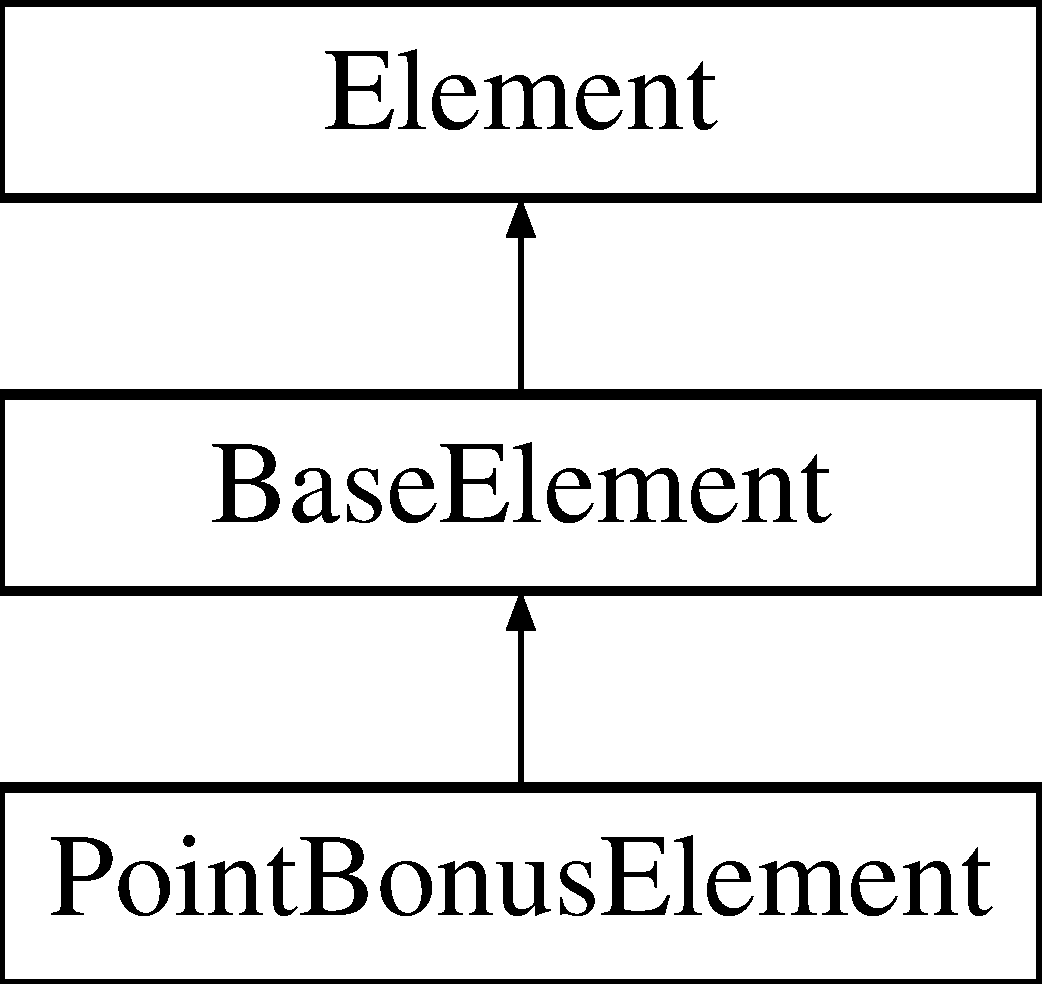
\includegraphics[height=3.000000cm]{classElement}
\end{center}
\end{figure}
\subsection*{Public Member Functions}
\begin{DoxyCompactItemize}
\item 
\hyperlink{classElement_ab0d0e20be9a36ae676202db753faeec9}{Element} ()
\begin{DoxyCompactList}\small\item\em Constructeur. \end{DoxyCompactList}\item 
\hyperlink{classElement_abd401e48661b56407c2d4c4da235f4ba}{Element} (int type)
\begin{DoxyCompactList}\small\item\em Surcharge du constructeur. \end{DoxyCompactList}\item 
\hyperlink{classElement_a4152d6fd18a1141be2592196c2c13d97}{Element} (bool random, int n\-\_\-el)
\begin{DoxyCompactList}\small\item\em Surcharge du constructeur. \end{DoxyCompactList}\item 
\hyperlink{classElement_a13d54ba9c08b6bec651402f1c2bb002c}{$\sim$\-Element} ()
\begin{DoxyCompactList}\small\item\em Destructeur. \end{DoxyCompactList}\item 
int \hyperlink{classElement_ae4b8bafd59a8e6bab7bb934679c200ac}{get\-Value} ()
\begin{DoxyCompactList}\small\item\em Accesseur de l'attribut value. \end{DoxyCompactList}\item 
int \hyperlink{classElement_a6414cb495f6b591c7ff9009682495c01}{get\-Money} ()
\begin{DoxyCompactList}\small\item\em accesseur de l'attribut Money \end{DoxyCompactList}\item 
int \hyperlink{classElement_a8bd9315dc4eb7b59f47410347375bf0e}{get\-Type} ()
\begin{DoxyCompactList}\small\item\em Accesseur de l'attribut type. \end{DoxyCompactList}\item 
void \hyperlink{classElement_a4629c727bd44fbae2a1a501edbc3a5f1}{set\-Type} (int type)
\begin{DoxyCompactList}\small\item\em Setteur de l'attribut type. \end{DoxyCompactList}\end{DoxyCompactItemize}
\subsection*{Protected Attributes}
\begin{DoxyCompactItemize}
\item 
\hypertarget{classElement_a4084eccd322ecebc24e906347595bc0a}{int \hyperlink{classElement_a4084eccd322ecebc24e906347595bc0a}{type\-\_\-}}\label{classElement_a4084eccd322ecebc24e906347595bc0a}

\begin{DoxyCompactList}\small\item\em Attribut type de l'élément. \end{DoxyCompactList}\item 
\hypertarget{classElement_ad9e52a612607b26d8595c195f013294e}{int \hyperlink{classElement_ad9e52a612607b26d8595c195f013294e}{value\-\_\-}}\label{classElement_ad9e52a612607b26d8595c195f013294e}

\begin{DoxyCompactList}\small\item\em Attribut value;. \end{DoxyCompactList}\item 
\hypertarget{classElement_a7302efe0ca5119b7bcb4f12e98f4b4ea}{int \hyperlink{classElement_a7302efe0ca5119b7bcb4f12e98f4b4ea}{money\-\_\-}}\label{classElement_a7302efe0ca5119b7bcb4f12e98f4b4ea}

\begin{DoxyCompactList}\small\item\em Attribut money;. \end{DoxyCompactList}\end{DoxyCompactItemize}


\subsection{Detailed Description}
La classe de gestion des éléments. 

\subsection{Constructor \& Destructor Documentation}
\hypertarget{classElement_ab0d0e20be9a36ae676202db753faeec9}{\index{Element@{Element}!Element@{Element}}
\index{Element@{Element}!Element@{Element}}
\subsubsection[{Element}]{\setlength{\rightskip}{0pt plus 5cm}Element\-::\-Element (
\begin{DoxyParamCaption}
{}
\end{DoxyParamCaption}
)}}\label{classElement_ab0d0e20be9a36ae676202db753faeec9}


Constructeur. 

Constructeur de la classe element \hypertarget{classElement_abd401e48661b56407c2d4c4da235f4ba}{\index{Element@{Element}!Element@{Element}}
\index{Element@{Element}!Element@{Element}}
\subsubsection[{Element}]{\setlength{\rightskip}{0pt plus 5cm}Element\-::\-Element (
\begin{DoxyParamCaption}
\item[{int}]{type}
\end{DoxyParamCaption}
)}}\label{classElement_abd401e48661b56407c2d4c4da235f4ba}


Surcharge du constructeur. 

Surcharge du constructeur de la classe \hyperlink{classElement}{Element}


\begin{DoxyParams}{Parameters}
{\em int} & type d'élément \\
\hline
\end{DoxyParams}
\hypertarget{classElement_a4152d6fd18a1141be2592196c2c13d97}{\index{Element@{Element}!Element@{Element}}
\index{Element@{Element}!Element@{Element}}
\subsubsection[{Element}]{\setlength{\rightskip}{0pt plus 5cm}Element\-::\-Element (
\begin{DoxyParamCaption}
\item[{bool}]{random, }
\item[{int}]{n\-\_\-el}
\end{DoxyParamCaption}
)}}\label{classElement_a4152d6fd18a1141be2592196c2c13d97}


Surcharge du constructeur. 

Surcharge du constructeur de la classe \hyperlink{classElement}{Element}


\begin{DoxyParams}{Parameters}
{\em booléen} & random pour la gestion de l'aléatoire \\
\hline
{\em entier} & nombre de type d'élément \\
\hline
\end{DoxyParams}
\hypertarget{classElement_a13d54ba9c08b6bec651402f1c2bb002c}{\index{Element@{Element}!$\sim$\-Element@{$\sim$\-Element}}
\index{$\sim$\-Element@{$\sim$\-Element}!Element@{Element}}
\subsubsection[{$\sim$\-Element}]{\setlength{\rightskip}{0pt plus 5cm}Element\-::$\sim$\-Element (
\begin{DoxyParamCaption}
{}
\end{DoxyParamCaption}
)}}\label{classElement_a13d54ba9c08b6bec651402f1c2bb002c}


Destructeur. 

Destructeur de la classe \hyperlink{classElement}{Element} 

\subsection{Member Function Documentation}
\hypertarget{classElement_a6414cb495f6b591c7ff9009682495c01}{\index{Element@{Element}!get\-Money@{get\-Money}}
\index{get\-Money@{get\-Money}!Element@{Element}}
\subsubsection[{get\-Money}]{\setlength{\rightskip}{0pt plus 5cm}int Element\-::get\-Money (
\begin{DoxyParamCaption}
{}
\end{DoxyParamCaption}
)}}\label{classElement_a6414cb495f6b591c7ff9009682495c01}


accesseur de l'attribut Money 

Méthode qui retourne la money de l'élément \begin{DoxyReturn}{Returns}
entier ; 
\end{DoxyReturn}
\hypertarget{classElement_a8bd9315dc4eb7b59f47410347375bf0e}{\index{Element@{Element}!get\-Type@{get\-Type}}
\index{get\-Type@{get\-Type}!Element@{Element}}
\subsubsection[{get\-Type}]{\setlength{\rightskip}{0pt plus 5cm}int Element\-::get\-Type (
\begin{DoxyParamCaption}
{}
\end{DoxyParamCaption}
)}}\label{classElement_a8bd9315dc4eb7b59f47410347375bf0e}


Accesseur de l'attribut type. 

Méthode qui retourne le type de l'élément \begin{DoxyReturn}{Returns}
entier le type de l'élément ; 
\end{DoxyReturn}
\hypertarget{classElement_ae4b8bafd59a8e6bab7bb934679c200ac}{\index{Element@{Element}!get\-Value@{get\-Value}}
\index{get\-Value@{get\-Value}!Element@{Element}}
\subsubsection[{get\-Value}]{\setlength{\rightskip}{0pt plus 5cm}int Element\-::get\-Value (
\begin{DoxyParamCaption}
{}
\end{DoxyParamCaption}
)}}\label{classElement_ae4b8bafd59a8e6bab7bb934679c200ac}


Accesseur de l'attribut value. 

Méthode qui retourne la valeur de l'élément \begin{DoxyReturn}{Returns}
entier, la valeur de l'élément 
\end{DoxyReturn}
\hypertarget{classElement_a4629c727bd44fbae2a1a501edbc3a5f1}{\index{Element@{Element}!set\-Type@{set\-Type}}
\index{set\-Type@{set\-Type}!Element@{Element}}
\subsubsection[{set\-Type}]{\setlength{\rightskip}{0pt plus 5cm}void Element\-::set\-Type (
\begin{DoxyParamCaption}
\item[{int}]{type}
\end{DoxyParamCaption}
)}}\label{classElement_a4629c727bd44fbae2a1a501edbc3a5f1}


Setteur de l'attribut type. 

Méthode qui affecte un nouveau type à l'élément 
\begin{DoxyParams}{Parameters}
{\em entier} & le nouveau type ; \\
\hline
\end{DoxyParams}


The documentation for this class was generated from the following file\-:\begin{DoxyCompactItemize}
\item 
include/Element.\-h\end{DoxyCompactItemize}

\hypertarget{classElementUI}{\section{Element\-U\-I Class Reference}
\label{classElementUI}\index{Element\-U\-I@{Element\-U\-I}}
}


Classe gérant l'affichage graphique des éléments.  




{\ttfamily \#include $<$Element\-U\-I.\-h$>$}

\subsection*{Public Member Functions}
\begin{DoxyCompactItemize}
\item 
\hyperlink{classElementUI_aba442422f66a0e5dd2c6720f49447a52}{Element\-U\-I} ()
\begin{DoxyCompactList}\small\item\em Constructeur. \end{DoxyCompactList}\item 
\hyperlink{classElementUI_a6b96a15cd508b01ba4df1fdb130e9094}{Element\-U\-I} (S\-D\-L\-\_\-\-Rect form, int x, int y, int type)
\begin{DoxyCompactList}\small\item\em Surcharge du constructeur. \end{DoxyCompactList}\item 
void \hyperlink{classElementUI_a6328f9ed38c5be1bbc40e767acc0557e}{draw} (S\-D\-L\-\_\-\-Surface $\ast$screen, S\-D\-L\-\_\-\-Surface $\ast$img)
\begin{DoxyCompactList}\small\item\em Méthode de \char`\"{}dessin\char`\"{}. \end{DoxyCompactList}\item 
bool \hyperlink{classElementUI_af050f41a37b8524b682e0fccff3532ef}{is\-On} (int x, int y)
\begin{DoxyCompactList}\small\item\em Méthode de vérification de coordonnée. \end{DoxyCompactList}\item 
bool \hyperlink{classElementUI_a08f605d10d4bcab0f62429816c20145c}{at\-Destination} ()
\begin{DoxyCompactList}\small\item\em Méthode de vérification de destination de l'élément. \end{DoxyCompactList}\item 
virtual \hyperlink{classElementUI_a3185daeef5db6386d4bef3cdad685b60}{$\sim$\-Element\-U\-I} ()
\begin{DoxyCompactList}\small\item\em Destructeur. \end{DoxyCompactList}\item 
S\-D\-L\-\_\-\-Rect \hyperlink{classElementUI_a95985a127a17afb4603bb4a43a571979}{get\-Form} ()
\begin{DoxyCompactList}\small\item\em Accesseur de la S\-D\-L\-\_\-\-Rec de la classe. \end{DoxyCompactList}\item 
int \hyperlink{classElementUI_a4e0d6c8ab7629d20e3d82c163fd616e8}{get\-X} ()
\begin{DoxyCompactList}\small\item\em Accesseur de l'abscisse de l'élément sur l'écran. \end{DoxyCompactList}\item 
int \hyperlink{classElementUI_a2d7985c4848780f45b2050ddd8c19126}{get\-Y} ()
\begin{DoxyCompactList}\small\item\em Accesseur de l'ordonnée de l'élément sur l'écran. \end{DoxyCompactList}\item 
int \hyperlink{classElementUI_ab0fded908da8a103f5f2ec1afff4cd15}{get\-Type} ()
\begin{DoxyCompactList}\small\item\em Accesseur du type de l'élément. \end{DoxyCompactList}\item 
int \hyperlink{classElementUI_a08b1c925bf4f500efadfc703b03dc3d5}{get\-Vel\-X} ()
\begin{DoxyCompactList}\small\item\em Accesseur de la vélocité x de l'élément sur l'écran. \end{DoxyCompactList}\item 
int \hyperlink{classElementUI_a4d7e54c2f05667aff3e8546ea3f30a10}{get\-Vel\-Y} ()
\begin{DoxyCompactList}\small\item\em Accesseur de la vélocité y de l'élément sur l'écran. \end{DoxyCompactList}\item 
int \hyperlink{classElementUI_abd5b1c0ad6bb7ebc50fc33e31fb94f0a}{get\-Dest\-X} ()
\begin{DoxyCompactList}\small\item\em Accesseur de la destination x de l'élément sur l'écran. \end{DoxyCompactList}\item 
int \hyperlink{classElementUI_a6e8c7e7467b8fafdd9e7c886b785ea51}{get\-Dest\-Y} ()
\begin{DoxyCompactList}\small\item\em Accesseur de la destination y de l'élément sur l'écran. \end{DoxyCompactList}\item 
void \hyperlink{classElementUI_afafbb62d1a13a9f56bf5f4ad78c20905}{set\-X} (int x)
\begin{DoxyCompactList}\small\item\em Setteur de l'abscisse x de l'élément. \end{DoxyCompactList}\item 
void \hyperlink{classElementUI_a13de120da5df1a81e0460fad5b88894e}{set\-Y} (int y)
\begin{DoxyCompactList}\small\item\em Setteur de l'ordonnée y de l'élément. \end{DoxyCompactList}\item 
void \hyperlink{classElementUI_a1c4fffc4b82d638e54af466149a6fd33}{set\-Type} (int type)
\begin{DoxyCompactList}\small\item\em Setteur du type de l'élément. \end{DoxyCompactList}\item 
void \hyperlink{classElementUI_a2cabdf9ffa98f640211dfdf42230d47e}{set\-Form} (S\-D\-L\-\_\-\-Rect form)
\begin{DoxyCompactList}\small\item\em Setteur de S\-D\-L\-\_\-\-Rec de l'élément. \end{DoxyCompactList}\item 
\hypertarget{classElementUI_a016963ca753305c277ce0d4f2aeaa2a2}{void {\bfseries set\-Form\-X} (int x)}\label{classElementUI_a016963ca753305c277ce0d4f2aeaa2a2}

\item 
\hypertarget{classElementUI_a151e22a2ac8858ad812da3bdd9ecefbc}{void {\bfseries set\-Form\-Y} (int y)}\label{classElementUI_a151e22a2ac8858ad812da3bdd9ecefbc}

\item 
void \hyperlink{classElementUI_abf1a5dc4177a2df976676507cc39e93e}{set\-Vel\-X} (int x)
\begin{DoxyCompactList}\small\item\em Setteur de la vélocité x de l'élément. \end{DoxyCompactList}\item 
void \hyperlink{classElementUI_ae1a5b66228e82a3fd3a9e30a86850b4b}{set\-Vel\-Y} (int y)
\begin{DoxyCompactList}\small\item\em Setteur de la vélocité y de l'élément. \end{DoxyCompactList}\item 
void \hyperlink{classElementUI_a9bd3e16eb12d10201079020869ca9b02}{set\-Dest\-X} (int x)
\begin{DoxyCompactList}\small\item\em Setteur de la destination x de l'élément sur l'écran. \end{DoxyCompactList}\item 
void \hyperlink{classElementUI_ad27f55f4c2cdb3f7d4b59ff8de619bfe}{set\-Dest\-Y} (int y)
\begin{DoxyCompactList}\small\item\em Setteur de la destination y de l'élément sur l'écran. \end{DoxyCompactList}\end{DoxyCompactItemize}


\subsection{Detailed Description}
Classe gérant l'affichage graphique des éléments. 

\subsection{Constructor \& Destructor Documentation}
\hypertarget{classElementUI_aba442422f66a0e5dd2c6720f49447a52}{\index{Element\-U\-I@{Element\-U\-I}!Element\-U\-I@{Element\-U\-I}}
\index{Element\-U\-I@{Element\-U\-I}!ElementUI@{Element\-U\-I}}
\subsubsection[{Element\-U\-I}]{\setlength{\rightskip}{0pt plus 5cm}Element\-U\-I\-::\-Element\-U\-I (
\begin{DoxyParamCaption}
{}
\end{DoxyParamCaption}
)}}\label{classElementUI_aba442422f66a0e5dd2c6720f49447a52}


Constructeur. 

Constructeur de la classe \hyperlink{classElementUI}{Element\-U\-I} \hypertarget{classElementUI_a6b96a15cd508b01ba4df1fdb130e9094}{\index{Element\-U\-I@{Element\-U\-I}!Element\-U\-I@{Element\-U\-I}}
\index{Element\-U\-I@{Element\-U\-I}!ElementUI@{Element\-U\-I}}
\subsubsection[{Element\-U\-I}]{\setlength{\rightskip}{0pt plus 5cm}Element\-U\-I\-::\-Element\-U\-I (
\begin{DoxyParamCaption}
\item[{S\-D\-L\-\_\-\-Rect}]{form, }
\item[{int}]{x, }
\item[{int}]{y, }
\item[{int}]{type}
\end{DoxyParamCaption}
)}}\label{classElementUI_a6b96a15cd508b01ba4df1fdb130e9094}


Surcharge du constructeur. 

Surcharge du constructeur de la classe \hyperlink{classElementUI}{Element\-U\-I}


\begin{DoxyParams}{Parameters}
{\em S\-D\-L\-\_\-\-Rect,paramètre} & des éléments \\
\hline
{\em entier,x} & (ligne) de l'élément dans la grille \\
\hline
{\em entier,y} & (colonne) de l'élément dans la grille \\
\hline
{\em entier,type} & de l'éléments \\
\hline
\end{DoxyParams}
\hypertarget{classElementUI_a3185daeef5db6386d4bef3cdad685b60}{\index{Element\-U\-I@{Element\-U\-I}!$\sim$\-Element\-U\-I@{$\sim$\-Element\-U\-I}}
\index{$\sim$\-Element\-U\-I@{$\sim$\-Element\-U\-I}!ElementUI@{Element\-U\-I}}
\subsubsection[{$\sim$\-Element\-U\-I}]{\setlength{\rightskip}{0pt plus 5cm}virtual Element\-U\-I\-::$\sim$\-Element\-U\-I (
\begin{DoxyParamCaption}
{}
\end{DoxyParamCaption}
)\hspace{0.3cm}{\ttfamily [virtual]}}}\label{classElementUI_a3185daeef5db6386d4bef3cdad685b60}


Destructeur. 

Destructeur de la classe \hyperlink{classElementUI}{Element\-U\-I} 

\subsection{Member Function Documentation}
\hypertarget{classElementUI_a08f605d10d4bcab0f62429816c20145c}{\index{Element\-U\-I@{Element\-U\-I}!at\-Destination@{at\-Destination}}
\index{at\-Destination@{at\-Destination}!ElementUI@{Element\-U\-I}}
\subsubsection[{at\-Destination}]{\setlength{\rightskip}{0pt plus 5cm}bool Element\-U\-I\-::at\-Destination (
\begin{DoxyParamCaption}
{}
\end{DoxyParamCaption}
)}}\label{classElementUI_a08f605d10d4bcab0f62429816c20145c}


Méthode de vérification de destination de l'élément. 

Méthode qui permet de vérifier si l'élément a atteind sa nouvelle \char`\"{}destination\char`\"{}

\begin{DoxyReturn}{Returns}
bool 
\end{DoxyReturn}
\hypertarget{classElementUI_a6328f9ed38c5be1bbc40e767acc0557e}{\index{Element\-U\-I@{Element\-U\-I}!draw@{draw}}
\index{draw@{draw}!ElementUI@{Element\-U\-I}}
\subsubsection[{draw}]{\setlength{\rightskip}{0pt plus 5cm}void Element\-U\-I\-::draw (
\begin{DoxyParamCaption}
\item[{S\-D\-L\-\_\-\-Surface $\ast$}]{screen, }
\item[{S\-D\-L\-\_\-\-Surface $\ast$}]{img}
\end{DoxyParamCaption}
)}}\label{classElementUI_a6328f9ed38c5be1bbc40e767acc0557e}


Méthode de \char`\"{}dessin\char`\"{}. 

Méthode qui permet de \char`\"{}dessiner\char`\"{} à l'écran l'élément


\begin{DoxyParams}{Parameters}
{\em S\-D\-L\-\_\-\-Surface,la} & surface sur laquelle on \char`\"{}dessine\char`\"{} l'élément \\
\hline
{\em S\-D\-L\-\_\-\-Surface,la} & surface image que l'on \char`\"{}colle\char`\"{} \\
\hline
\end{DoxyParams}
\hypertarget{classElementUI_abd5b1c0ad6bb7ebc50fc33e31fb94f0a}{\index{Element\-U\-I@{Element\-U\-I}!get\-Dest\-X@{get\-Dest\-X}}
\index{get\-Dest\-X@{get\-Dest\-X}!ElementUI@{Element\-U\-I}}
\subsubsection[{get\-Dest\-X}]{\setlength{\rightskip}{0pt plus 5cm}int Element\-U\-I\-::get\-Dest\-X (
\begin{DoxyParamCaption}
{}
\end{DoxyParamCaption}
)}}\label{classElementUI_abd5b1c0ad6bb7ebc50fc33e31fb94f0a}


Accesseur de la destination x de l'élément sur l'écran. 

Méthode qui retourne la destination x de l'élément sur l'écran

\begin{DoxyReturn}{Returns}
entier, la destination x 
\end{DoxyReturn}
\hypertarget{classElementUI_a6e8c7e7467b8fafdd9e7c886b785ea51}{\index{Element\-U\-I@{Element\-U\-I}!get\-Dest\-Y@{get\-Dest\-Y}}
\index{get\-Dest\-Y@{get\-Dest\-Y}!ElementUI@{Element\-U\-I}}
\subsubsection[{get\-Dest\-Y}]{\setlength{\rightskip}{0pt plus 5cm}int Element\-U\-I\-::get\-Dest\-Y (
\begin{DoxyParamCaption}
{}
\end{DoxyParamCaption}
)}}\label{classElementUI_a6e8c7e7467b8fafdd9e7c886b785ea51}


Accesseur de la destination y de l'élément sur l'écran. 

Méthode qui retourne la destination y de l'élément sur l'écran

\begin{DoxyReturn}{Returns}
entier, la destination y 
\end{DoxyReturn}
\hypertarget{classElementUI_a95985a127a17afb4603bb4a43a571979}{\index{Element\-U\-I@{Element\-U\-I}!get\-Form@{get\-Form}}
\index{get\-Form@{get\-Form}!ElementUI@{Element\-U\-I}}
\subsubsection[{get\-Form}]{\setlength{\rightskip}{0pt plus 5cm}S\-D\-L\-\_\-\-Rect Element\-U\-I\-::get\-Form (
\begin{DoxyParamCaption}
{}
\end{DoxyParamCaption}
)}}\label{classElementUI_a95985a127a17afb4603bb4a43a571979}


Accesseur de la S\-D\-L\-\_\-\-Rec de la classe. 

Méthode qui retourne la S\-D\-L\-\_\-\-Rec de la classe \hyperlink{classElementUI}{Element\-U\-I}

\begin{DoxyReturn}{Returns}
S\-Dl\-\_\-\-Rec; 
\end{DoxyReturn}
\hypertarget{classElementUI_ab0fded908da8a103f5f2ec1afff4cd15}{\index{Element\-U\-I@{Element\-U\-I}!get\-Type@{get\-Type}}
\index{get\-Type@{get\-Type}!ElementUI@{Element\-U\-I}}
\subsubsection[{get\-Type}]{\setlength{\rightskip}{0pt plus 5cm}int Element\-U\-I\-::get\-Type (
\begin{DoxyParamCaption}
{}
\end{DoxyParamCaption}
)}}\label{classElementUI_ab0fded908da8a103f5f2ec1afff4cd15}


Accesseur du type de l'élément. 

Méthode qui retourne l'abscisse de l'élément

\begin{DoxyReturn}{Returns}
entier, le type 
\end{DoxyReturn}
\hypertarget{classElementUI_a08b1c925bf4f500efadfc703b03dc3d5}{\index{Element\-U\-I@{Element\-U\-I}!get\-Vel\-X@{get\-Vel\-X}}
\index{get\-Vel\-X@{get\-Vel\-X}!ElementUI@{Element\-U\-I}}
\subsubsection[{get\-Vel\-X}]{\setlength{\rightskip}{0pt plus 5cm}int Element\-U\-I\-::get\-Vel\-X (
\begin{DoxyParamCaption}
{}
\end{DoxyParamCaption}
)}}\label{classElementUI_a08b1c925bf4f500efadfc703b03dc3d5}


Accesseur de la vélocité x de l'élément sur l'écran. 

Méthode qui retourne la vélocité x de l'élément sur l'écran

\begin{DoxyReturn}{Returns}
entier, la vélocité x 
\end{DoxyReturn}
\hypertarget{classElementUI_a4d7e54c2f05667aff3e8546ea3f30a10}{\index{Element\-U\-I@{Element\-U\-I}!get\-Vel\-Y@{get\-Vel\-Y}}
\index{get\-Vel\-Y@{get\-Vel\-Y}!ElementUI@{Element\-U\-I}}
\subsubsection[{get\-Vel\-Y}]{\setlength{\rightskip}{0pt plus 5cm}int Element\-U\-I\-::get\-Vel\-Y (
\begin{DoxyParamCaption}
{}
\end{DoxyParamCaption}
)}}\label{classElementUI_a4d7e54c2f05667aff3e8546ea3f30a10}


Accesseur de la vélocité y de l'élément sur l'écran. 

Méthode qui retourne la vélocité y de l'élément sur l'écran

\begin{DoxyReturn}{Returns}
entier, la vélocité y 
\end{DoxyReturn}
\hypertarget{classElementUI_a4e0d6c8ab7629d20e3d82c163fd616e8}{\index{Element\-U\-I@{Element\-U\-I}!get\-X@{get\-X}}
\index{get\-X@{get\-X}!ElementUI@{Element\-U\-I}}
\subsubsection[{get\-X}]{\setlength{\rightskip}{0pt plus 5cm}int Element\-U\-I\-::get\-X (
\begin{DoxyParamCaption}
{}
\end{DoxyParamCaption}
)}}\label{classElementUI_a4e0d6c8ab7629d20e3d82c163fd616e8}


Accesseur de l'abscisse de l'élément sur l'écran. 

Méthode qui retourne l'abscisse de l'élément sur l'écran

\begin{DoxyReturn}{Returns}
entier, x l'abscisse 
\end{DoxyReturn}
\hypertarget{classElementUI_a2d7985c4848780f45b2050ddd8c19126}{\index{Element\-U\-I@{Element\-U\-I}!get\-Y@{get\-Y}}
\index{get\-Y@{get\-Y}!ElementUI@{Element\-U\-I}}
\subsubsection[{get\-Y}]{\setlength{\rightskip}{0pt plus 5cm}int Element\-U\-I\-::get\-Y (
\begin{DoxyParamCaption}
{}
\end{DoxyParamCaption}
)}}\label{classElementUI_a2d7985c4848780f45b2050ddd8c19126}


Accesseur de l'ordonnée de l'élément sur l'écran. 

Méthode qui retourne l'ordonnée de l'élément sur l'écran

\begin{DoxyReturn}{Returns}
entier, y l'ordonnée 
\end{DoxyReturn}
\hypertarget{classElementUI_af050f41a37b8524b682e0fccff3532ef}{\index{Element\-U\-I@{Element\-U\-I}!is\-On@{is\-On}}
\index{is\-On@{is\-On}!ElementUI@{Element\-U\-I}}
\subsubsection[{is\-On}]{\setlength{\rightskip}{0pt plus 5cm}bool Element\-U\-I\-::is\-On (
\begin{DoxyParamCaption}
\item[{int}]{x, }
\item[{int}]{y}
\end{DoxyParamCaption}
)}}\label{classElementUI_af050f41a37b8524b682e0fccff3532ef}


Méthode de vérification de coordonnée. 

méthode qui permet vérifier le passage de la souris sur l'élément


\begin{DoxyParams}{Parameters}
{\em entier,x} & l'abscisse de la souris sur l'écran \\
\hline
{\em entier,y} & l'ordonnée de la souris sur l'écran \\
\hline
\end{DoxyParams}
\begin{DoxyReturn}{Returns}
booléen, true si la souris est sur l'élément false sinon 
\end{DoxyReturn}
\hypertarget{classElementUI_a9bd3e16eb12d10201079020869ca9b02}{\index{Element\-U\-I@{Element\-U\-I}!set\-Dest\-X@{set\-Dest\-X}}
\index{set\-Dest\-X@{set\-Dest\-X}!ElementUI@{Element\-U\-I}}
\subsubsection[{set\-Dest\-X}]{\setlength{\rightskip}{0pt plus 5cm}void Element\-U\-I\-::set\-Dest\-X (
\begin{DoxyParamCaption}
\item[{int}]{x}
\end{DoxyParamCaption}
)}}\label{classElementUI_a9bd3e16eb12d10201079020869ca9b02}


Setteur de la destination x de l'élément sur l'écran. 

Méthode qui retourne la destination x de l'élément sur l'écran


\begin{DoxyParams}{Parameters}
{\em entier} & \\
\hline
\end{DoxyParams}
\hypertarget{classElementUI_ad27f55f4c2cdb3f7d4b59ff8de619bfe}{\index{Element\-U\-I@{Element\-U\-I}!set\-Dest\-Y@{set\-Dest\-Y}}
\index{set\-Dest\-Y@{set\-Dest\-Y}!ElementUI@{Element\-U\-I}}
\subsubsection[{set\-Dest\-Y}]{\setlength{\rightskip}{0pt plus 5cm}void Element\-U\-I\-::set\-Dest\-Y (
\begin{DoxyParamCaption}
\item[{int}]{y}
\end{DoxyParamCaption}
)}}\label{classElementUI_ad27f55f4c2cdb3f7d4b59ff8de619bfe}


Setteur de la destination y de l'élément sur l'écran. 

Méthode qui retourne la destination y de l'élément sur l'écran


\begin{DoxyParams}{Parameters}
{\em entier} & \\
\hline
\end{DoxyParams}
\hypertarget{classElementUI_a2cabdf9ffa98f640211dfdf42230d47e}{\index{Element\-U\-I@{Element\-U\-I}!set\-Form@{set\-Form}}
\index{set\-Form@{set\-Form}!ElementUI@{Element\-U\-I}}
\subsubsection[{set\-Form}]{\setlength{\rightskip}{0pt plus 5cm}void Element\-U\-I\-::set\-Form (
\begin{DoxyParamCaption}
\item[{S\-D\-L\-\_\-\-Rect}]{form}
\end{DoxyParamCaption}
)}}\label{classElementUI_a2cabdf9ffa98f640211dfdf42230d47e}


Setteur de S\-D\-L\-\_\-\-Rec de l'élément. 

Méthode qui affecte la nouvelle S\-D\-L\-\_\-\-Rec de l'élément \hypertarget{classElementUI_a1c4fffc4b82d638e54af466149a6fd33}{\index{Element\-U\-I@{Element\-U\-I}!set\-Type@{set\-Type}}
\index{set\-Type@{set\-Type}!ElementUI@{Element\-U\-I}}
\subsubsection[{set\-Type}]{\setlength{\rightskip}{0pt plus 5cm}void Element\-U\-I\-::set\-Type (
\begin{DoxyParamCaption}
\item[{int}]{type}
\end{DoxyParamCaption}
)}}\label{classElementUI_a1c4fffc4b82d638e54af466149a6fd33}


Setteur du type de l'élément. 

Méthode qui affecte le nouveau type de l'élément \hypertarget{classElementUI_abf1a5dc4177a2df976676507cc39e93e}{\index{Element\-U\-I@{Element\-U\-I}!set\-Vel\-X@{set\-Vel\-X}}
\index{set\-Vel\-X@{set\-Vel\-X}!ElementUI@{Element\-U\-I}}
\subsubsection[{set\-Vel\-X}]{\setlength{\rightskip}{0pt plus 5cm}void Element\-U\-I\-::set\-Vel\-X (
\begin{DoxyParamCaption}
\item[{int}]{x}
\end{DoxyParamCaption}
)}}\label{classElementUI_abf1a5dc4177a2df976676507cc39e93e}


Setteur de la vélocité x de l'élément. 

Méthode qui affecte la vélocité x de l'élément


\begin{DoxyParams}{Parameters}
{\em entier} & \\
\hline
\end{DoxyParams}
\hypertarget{classElementUI_ae1a5b66228e82a3fd3a9e30a86850b4b}{\index{Element\-U\-I@{Element\-U\-I}!set\-Vel\-Y@{set\-Vel\-Y}}
\index{set\-Vel\-Y@{set\-Vel\-Y}!ElementUI@{Element\-U\-I}}
\subsubsection[{set\-Vel\-Y}]{\setlength{\rightskip}{0pt plus 5cm}void Element\-U\-I\-::set\-Vel\-Y (
\begin{DoxyParamCaption}
\item[{int}]{y}
\end{DoxyParamCaption}
)}}\label{classElementUI_ae1a5b66228e82a3fd3a9e30a86850b4b}


Setteur de la vélocité y de l'élément. 

Méthode qui affecte la vélocité y de l'élément


\begin{DoxyParams}{Parameters}
{\em entier} & \\
\hline
\end{DoxyParams}
\hypertarget{classElementUI_afafbb62d1a13a9f56bf5f4ad78c20905}{\index{Element\-U\-I@{Element\-U\-I}!set\-X@{set\-X}}
\index{set\-X@{set\-X}!ElementUI@{Element\-U\-I}}
\subsubsection[{set\-X}]{\setlength{\rightskip}{0pt plus 5cm}void Element\-U\-I\-::set\-X (
\begin{DoxyParamCaption}
\item[{int}]{x}
\end{DoxyParamCaption}
)}}\label{classElementUI_afafbb62d1a13a9f56bf5f4ad78c20905}


Setteur de l'abscisse x de l'élément. 

Méthode qui affecte la nouvelle abscisse à l'élément \hypertarget{classElementUI_a13de120da5df1a81e0460fad5b88894e}{\index{Element\-U\-I@{Element\-U\-I}!set\-Y@{set\-Y}}
\index{set\-Y@{set\-Y}!ElementUI@{Element\-U\-I}}
\subsubsection[{set\-Y}]{\setlength{\rightskip}{0pt plus 5cm}void Element\-U\-I\-::set\-Y (
\begin{DoxyParamCaption}
\item[{int}]{y}
\end{DoxyParamCaption}
)}}\label{classElementUI_a13de120da5df1a81e0460fad5b88894e}


Setteur de l'ordonnée y de l'élément. 

Méthode qui affecte la nouvelle ordonnée y de l'élément 

The documentation for this class was generated from the following file\-:\begin{DoxyCompactItemize}
\item 
include/Element\-U\-I.\-h\end{DoxyCompactItemize}

\hypertarget{classEngine}{\section{Engine Class Reference}
\label{classEngine}\index{Engine@{Engine}}
}


La classe \hyperlink{classEngine}{Engine}, moteur du jeu.  




{\ttfamily \#include $<$Engine.\-h$>$}

\subsection*{Public Member Functions}
\begin{DoxyCompactItemize}
\item 
virtual \hyperlink{classEngine_a41f2d854040e17d9c4d7b324a4bfbf39}{$\sim$\-Engine} ()
\begin{DoxyCompactList}\small\item\em Destructeur. \end{DoxyCompactList}\item 
void \hyperlink{classEngine_ab44d76e2ff6057e73d6210cf9af0d89e}{init} ()
\begin{DoxyCompactList}\small\item\em Initialisation de \hyperlink{classEngine}{Engine}. \end{DoxyCompactList}\item 
\hypertarget{classEngine_af81ae123a517a8d15cff3c6a091d5050}{void {\bfseries event} ()}\label{classEngine_af81ae123a517a8d15cff3c6a091d5050}

\item 
\hypertarget{classEngine_a7960743aefd62e846e7f3cd92c18bc73}{void {\bfseries render} ()}\label{classEngine_a7960743aefd62e846e7f3cd92c18bc73}

\item 
void \hyperlink{classEngine_a0271409e3d247a540e1f267627dded4e}{set\-Screen} (\hyperlink{classScreen}{Screen} $\ast$screen)
\begin{DoxyCompactList}\small\item\em Setteur de l'attribut screen l'écran principal. \end{DoxyCompactList}\item 
void \hyperlink{classEngine_aa2c787d89892ad75da20ce4d4c5561de}{set\-Grid\-Mode} (\hyperlink{classGridMode}{Grid\-Mode} $\ast$grid\-Mode)
\begin{DoxyCompactList}\small\item\em Setteur de l'attribut grid\-Mode. \end{DoxyCompactList}\item 
\hyperlink{classGrid}{Grid} $\ast$ \hyperlink{classEngine_ad03dd023db9027a1268a65fd04295e66}{get\-Grid} ()
\begin{DoxyCompactList}\small\item\em Accesseur de l'attribut grid\-Mode. \end{DoxyCompactList}\item 
\hyperlink{classScreen}{Screen} $\ast$ \hyperlink{classEngine_af620e94fcf485aaec49d1dde7d6f389f}{get\-Screen} ()
\begin{DoxyCompactList}\small\item\em Accesseur de l'attribut screen. \end{DoxyCompactList}\item 
S\-D\-L\-\_\-\-Surface $\ast$ \hyperlink{classEngine_a0bfca2729728e42d6ac31b77e20a9dae}{get\-S\-D\-Lscreen} ()
\begin{DoxyCompactList}\small\item\em Accesseur de l'attribut S\-Dlscreen. \end{DoxyCompactList}\item 
\hyperlink{classScreen}{Screen} $\ast$ \hyperlink{classEngine_a212ec7844a597a360b03d8a125e53f5e}{get\-Menu\-Screen} ()
\begin{DoxyCompactList}\small\item\em Accesseur de l'attribut menu\-Screen. \end{DoxyCompactList}\item 
\hyperlink{classScreen}{Screen} $\ast$ \hyperlink{classEngine_af6d0e82cecee32853a37ebdb9ea9fcc1}{get\-Game\-Screen} ()
\begin{DoxyCompactList}\small\item\em Accesseur de l'attribut game\-Screen. \end{DoxyCompactList}\item 
void \hyperlink{classEngine_a4a788fd99f4c92744b31085febb02c11}{set\-Event} (S\-D\-L\-\_\-\-Event $\ast$event)
\begin{DoxyCompactList}\small\item\em Setteur de l'attribut event. \end{DoxyCompactList}\item 
void \hyperlink{classEngine_a1564feb179849566523a67cfc344c613}{set\-Loop} (bool $\ast$loop)
\begin{DoxyCompactList}\small\item\em setteur de l'attribut Loop \end{DoxyCompactList}\item 
void \hyperlink{classEngine_a44eb0e03051e9057c1301f24d0551b20}{set\-S\-D\-Lscreen} (S\-D\-L\-\_\-\-Surface $\ast$new\-Screen)
\begin{DoxyCompactList}\small\item\em setteur de l'attribut S\-D\-Lscreen \end{DoxyCompactList}\end{DoxyCompactItemize}
\subsection*{Static Public Member Functions}
\begin{DoxyCompactItemize}
\item 
static \hyperlink{classEngine}{Engine} $\ast$ \hyperlink{classEngine_a5fd3090d4ac77870893bd27ce5623c5c}{get\-Instance} ()
\begin{DoxyCompactList}\small\item\em Méthode du Singleton pour obtenir une seul instance de \hyperlink{classEngine}{Engine}. \end{DoxyCompactList}\end{DoxyCompactItemize}


\subsection{Detailed Description}
La classe \hyperlink{classEngine}{Engine}, moteur du jeu. 

\subsection{Constructor \& Destructor Documentation}
\hypertarget{classEngine_a41f2d854040e17d9c4d7b324a4bfbf39}{\index{Engine@{Engine}!$\sim$\-Engine@{$\sim$\-Engine}}
\index{$\sim$\-Engine@{$\sim$\-Engine}!Engine@{Engine}}
\subsubsection[{$\sim$\-Engine}]{\setlength{\rightskip}{0pt plus 5cm}virtual Engine\-::$\sim$\-Engine (
\begin{DoxyParamCaption}
{}
\end{DoxyParamCaption}
)\hspace{0.3cm}{\ttfamily [virtual]}}}\label{classEngine_a41f2d854040e17d9c4d7b324a4bfbf39}


Destructeur. 

Destructeur de la classe \hyperlink{classEngine}{Engine} 

\subsection{Member Function Documentation}
\hypertarget{classEngine_af6d0e82cecee32853a37ebdb9ea9fcc1}{\index{Engine@{Engine}!get\-Game\-Screen@{get\-Game\-Screen}}
\index{get\-Game\-Screen@{get\-Game\-Screen}!Engine@{Engine}}
\subsubsection[{get\-Game\-Screen}]{\setlength{\rightskip}{0pt plus 5cm}{\bf Screen}$\ast$ Engine\-::get\-Game\-Screen (
\begin{DoxyParamCaption}
{}
\end{DoxyParamCaption}
)}}\label{classEngine_af6d0e82cecee32853a37ebdb9ea9fcc1}


Accesseur de l'attribut game\-Screen. 

Méthode qui retourne l'attibut écran de jeux

\begin{DoxyReturn}{Returns}
screen , l'écran de jeux 
\end{DoxyReturn}
\hypertarget{classEngine_ad03dd023db9027a1268a65fd04295e66}{\index{Engine@{Engine}!get\-Grid@{get\-Grid}}
\index{get\-Grid@{get\-Grid}!Engine@{Engine}}
\subsubsection[{get\-Grid}]{\setlength{\rightskip}{0pt plus 5cm}{\bf Grid}$\ast$ Engine\-::get\-Grid (
\begin{DoxyParamCaption}
{}
\end{DoxyParamCaption}
)}}\label{classEngine_ad03dd023db9027a1268a65fd04295e66}


Accesseur de l'attribut grid\-Mode. 

Méthode qui retourne la grille du jeux

\begin{DoxyReturn}{Returns}
\hyperlink{classGrid}{Grid}, la grille 
\end{DoxyReturn}
\hypertarget{classEngine_a5fd3090d4ac77870893bd27ce5623c5c}{\index{Engine@{Engine}!get\-Instance@{get\-Instance}}
\index{get\-Instance@{get\-Instance}!Engine@{Engine}}
\subsubsection[{get\-Instance}]{\setlength{\rightskip}{0pt plus 5cm}static {\bf Engine}$\ast$ Engine\-::get\-Instance (
\begin{DoxyParamCaption}
{}
\end{DoxyParamCaption}
)\hspace{0.3cm}{\ttfamily [inline]}, {\ttfamily [static]}}}\label{classEngine_a5fd3090d4ac77870893bd27ce5623c5c}


Méthode du Singleton pour obtenir une seul instance de \hyperlink{classEngine}{Engine}. 

\begin{DoxyReturn}{Returns}
\hyperlink{classEngine}{Engine} l'instance de la classe 
\end{DoxyReturn}
\hypertarget{classEngine_a212ec7844a597a360b03d8a125e53f5e}{\index{Engine@{Engine}!get\-Menu\-Screen@{get\-Menu\-Screen}}
\index{get\-Menu\-Screen@{get\-Menu\-Screen}!Engine@{Engine}}
\subsubsection[{get\-Menu\-Screen}]{\setlength{\rightskip}{0pt plus 5cm}{\bf Screen}$\ast$ Engine\-::get\-Menu\-Screen (
\begin{DoxyParamCaption}
{}
\end{DoxyParamCaption}
)}}\label{classEngine_a212ec7844a597a360b03d8a125e53f5e}


Accesseur de l'attribut menu\-Screen. 

Méthode qui retourne l'attribut écran de menu

\begin{DoxyReturn}{Returns}
screen , l'écran du menu 
\end{DoxyReturn}
\hypertarget{classEngine_af620e94fcf485aaec49d1dde7d6f389f}{\index{Engine@{Engine}!get\-Screen@{get\-Screen}}
\index{get\-Screen@{get\-Screen}!Engine@{Engine}}
\subsubsection[{get\-Screen}]{\setlength{\rightskip}{0pt plus 5cm}{\bf Screen}$\ast$ Engine\-::get\-Screen (
\begin{DoxyParamCaption}
{}
\end{DoxyParamCaption}
)}}\label{classEngine_af620e94fcf485aaec49d1dde7d6f389f}


Accesseur de l'attribut screen. 

Méthode qui retourne l'écran courant

\begin{DoxyReturn}{Returns}
\hyperlink{classScreen}{Screen} , l'écran courant 
\end{DoxyReturn}
\hypertarget{classEngine_a0bfca2729728e42d6ac31b77e20a9dae}{\index{Engine@{Engine}!get\-S\-D\-Lscreen@{get\-S\-D\-Lscreen}}
\index{get\-S\-D\-Lscreen@{get\-S\-D\-Lscreen}!Engine@{Engine}}
\subsubsection[{get\-S\-D\-Lscreen}]{\setlength{\rightskip}{0pt plus 5cm}S\-D\-L\-\_\-\-Surface$\ast$ Engine\-::get\-S\-D\-Lscreen (
\begin{DoxyParamCaption}
{}
\end{DoxyParamCaption}
)}}\label{classEngine_a0bfca2729728e42d6ac31b77e20a9dae}


Accesseur de l'attribut S\-Dlscreen. 

Méthode qui retourne la S\-D\-L\-\_\-\-Surface

\begin{DoxyReturn}{Returns}
S\-D\-L\-\_\-\-Surface , S\-D\-Lscreen 
\end{DoxyReturn}
\hypertarget{classEngine_ab44d76e2ff6057e73d6210cf9af0d89e}{\index{Engine@{Engine}!init@{init}}
\index{init@{init}!Engine@{Engine}}
\subsubsection[{init}]{\setlength{\rightskip}{0pt plus 5cm}void Engine\-::init (
\begin{DoxyParamCaption}
{}
\end{DoxyParamCaption}
)}}\label{classEngine_ab44d76e2ff6057e73d6210cf9af0d89e}


Initialisation de \hyperlink{classEngine}{Engine}. 

Méthode qui initialise les attributs de \hyperlink{classEngine}{Engine} \hypertarget{classEngine_a4a788fd99f4c92744b31085febb02c11}{\index{Engine@{Engine}!set\-Event@{set\-Event}}
\index{set\-Event@{set\-Event}!Engine@{Engine}}
\subsubsection[{set\-Event}]{\setlength{\rightskip}{0pt plus 5cm}void Engine\-::set\-Event (
\begin{DoxyParamCaption}
\item[{S\-D\-L\-\_\-\-Event $\ast$}]{event}
\end{DoxyParamCaption}
)}}\label{classEngine_a4a788fd99f4c92744b31085febb02c11}


Setteur de l'attribut event. 

Méthode qui affecte la nouvelle valeur de event \hypertarget{classEngine_aa2c787d89892ad75da20ce4d4c5561de}{\index{Engine@{Engine}!set\-Grid\-Mode@{set\-Grid\-Mode}}
\index{set\-Grid\-Mode@{set\-Grid\-Mode}!Engine@{Engine}}
\subsubsection[{set\-Grid\-Mode}]{\setlength{\rightskip}{0pt plus 5cm}void Engine\-::set\-Grid\-Mode (
\begin{DoxyParamCaption}
\item[{{\bf Grid\-Mode} $\ast$}]{grid\-Mode}
\end{DoxyParamCaption}
)}}\label{classEngine_aa2c787d89892ad75da20ce4d4c5561de}


Setteur de l'attribut grid\-Mode. 

Méthode qui affecte le mode de jeux \hypertarget{classEngine_a1564feb179849566523a67cfc344c613}{\index{Engine@{Engine}!set\-Loop@{set\-Loop}}
\index{set\-Loop@{set\-Loop}!Engine@{Engine}}
\subsubsection[{set\-Loop}]{\setlength{\rightskip}{0pt plus 5cm}void Engine\-::set\-Loop (
\begin{DoxyParamCaption}
\item[{bool $\ast$}]{loop}
\end{DoxyParamCaption}
)}}\label{classEngine_a1564feb179849566523a67cfc344c613}


setteur de l'attribut Loop 

méthode qui affecte la nouvelle valeur de la boucle de jeux \hypertarget{classEngine_a0271409e3d247a540e1f267627dded4e}{\index{Engine@{Engine}!set\-Screen@{set\-Screen}}
\index{set\-Screen@{set\-Screen}!Engine@{Engine}}
\subsubsection[{set\-Screen}]{\setlength{\rightskip}{0pt plus 5cm}void Engine\-::set\-Screen (
\begin{DoxyParamCaption}
\item[{{\bf Screen} $\ast$}]{screen}
\end{DoxyParamCaption}
)}}\label{classEngine_a0271409e3d247a540e1f267627dded4e}


Setteur de l'attribut screen l'écran principal. 

Méthode qui affecte le nouvelle écran principal au moteur \hypertarget{classEngine_a44eb0e03051e9057c1301f24d0551b20}{\index{Engine@{Engine}!set\-S\-D\-Lscreen@{set\-S\-D\-Lscreen}}
\index{set\-S\-D\-Lscreen@{set\-S\-D\-Lscreen}!Engine@{Engine}}
\subsubsection[{set\-S\-D\-Lscreen}]{\setlength{\rightskip}{0pt plus 5cm}void Engine\-::set\-S\-D\-Lscreen (
\begin{DoxyParamCaption}
\item[{S\-D\-L\-\_\-\-Surface $\ast$}]{new\-Screen}
\end{DoxyParamCaption}
)}}\label{classEngine_a44eb0e03051e9057c1301f24d0551b20}


setteur de l'attribut S\-D\-Lscreen 

méthode qui affecte la nouvelle valeur de S\-D\-Lscreen

\begin{DoxyReturn}{Returns}
screen , l'écran de jeux 
\end{DoxyReturn}


The documentation for this class was generated from the following file\-:\begin{DoxyCompactItemize}
\item 
include/Engine.\-h\end{DoxyCompactItemize}

\hypertarget{classGameScreen}{\section{Game\-Screen Class Reference}
\label{classGameScreen}\index{Game\-Screen@{Game\-Screen}}
}


La classe \hyperlink{classGameScreen}{Game\-Screen}, gestion de l'écran de jeu implémente l'interface \hyperlink{classScreen}{Screen}.  




{\ttfamily \#include $<$Game\-Screen.\-h$>$}

Inheritance diagram for Game\-Screen\-:\begin{figure}[H]
\begin{center}
\leavevmode
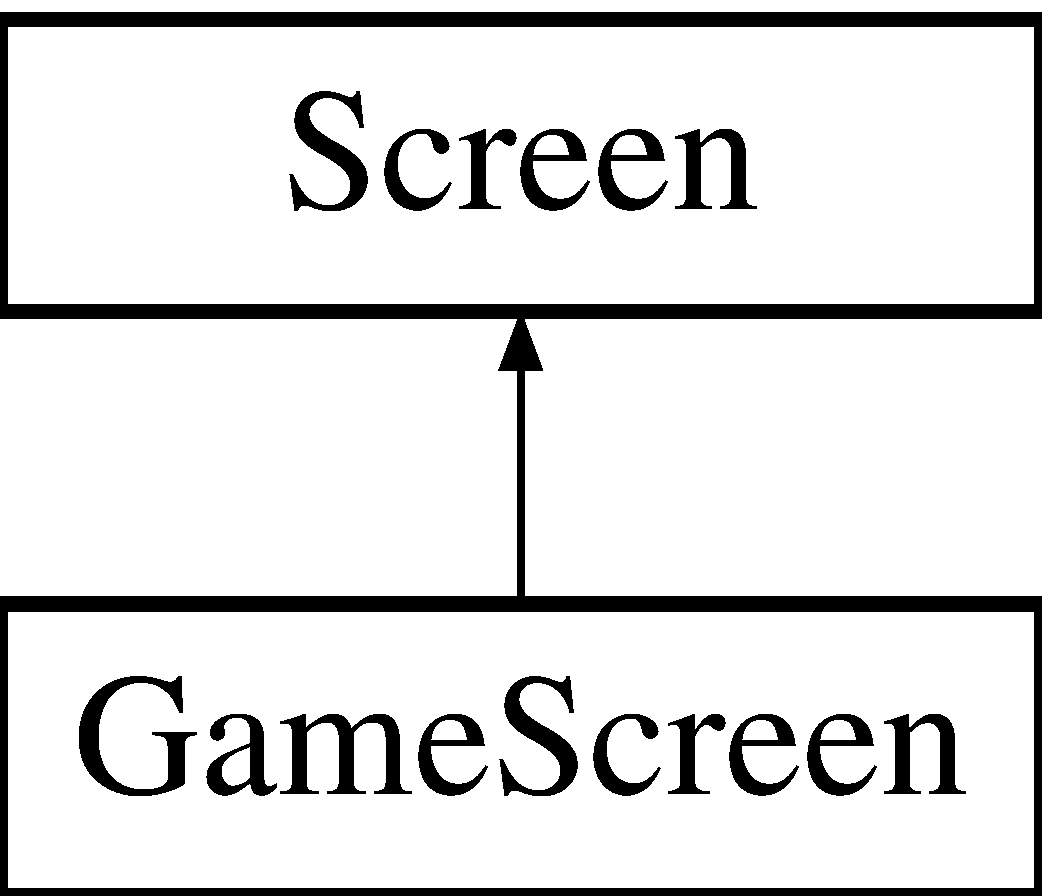
\includegraphics[height=2.000000cm]{classGameScreen}
\end{center}
\end{figure}
\subsection*{Public Member Functions}
\begin{DoxyCompactItemize}
\item 
\hyperlink{classGameScreen_ae8cfcd6a8b7a66d71b93ff67aae97548}{Game\-Screen} (\hyperlink{classEngine}{Engine} $\ast$engine)
\begin{DoxyCompactList}\small\item\em Constructeur. \end{DoxyCompactList}\item 
virtual \hyperlink{classGameScreen_a6e5c5a19486f4f74086e976d80f3fa14}{$\sim$\-Game\-Screen} ()
\begin{DoxyCompactList}\small\item\em Destructeur. \end{DoxyCompactList}\item 
void \hyperlink{classGameScreen_a43a2a1a9c28f8e2892ae3d91e1dcfa1f}{show} (S\-D\-L\-\_\-\-Surface $\ast$screen)
\begin{DoxyCompactList}\small\item\em Méthode show. \end{DoxyCompactList}\item 
void \hyperlink{classGameScreen_a8f4d95f64f07e01b4ebe35b31b39acb7}{render} (S\-D\-L\-\_\-\-Surface $\ast$screen)
\begin{DoxyCompactList}\small\item\em methode render \end{DoxyCompactList}\item 
void \hyperlink{classGameScreen_a0b4bad004b986f9aeed9b8f69606c11b}{resize} (S\-D\-L\-\_\-\-Surface $\ast$screen)
\begin{DoxyCompactList}\small\item\em methode resize \end{DoxyCompactList}\item 
void \hyperlink{classGameScreen_ac818a2dc8c094fc2bb23ceb0a0a53cf3}{hide} (S\-D\-L\-\_\-\-Surface $\ast$screen)
\begin{DoxyCompactList}\small\item\em Méthode hide. \end{DoxyCompactList}\item 
void \hyperlink{classGameScreen_a542fcc8ed203427ea442bb2f52406a91}{event} (S\-D\-L\-\_\-\-Event $\ast$event, bool $\ast$loop)
\begin{DoxyCompactList}\small\item\em Méthode event. \end{DoxyCompactList}\item 
void \hyperlink{classGameScreen_a46f96d4b6a0bbd02e83ce25318912c47}{mouse\-Click} (int x, int y)
\begin{DoxyCompactList}\small\item\em Méthode mouse\-Click. \end{DoxyCompactList}\item 
void \hyperlink{classGameScreen_ab6e0880af2f79d9a831910a7381de15d}{update\-Elements} ()
\begin{DoxyCompactList}\small\item\em methode update\-Elements \end{DoxyCompactList}\item 
void \hyperlink{classGameScreen_a20181c29cfa2dc257b642658fe386480}{set\-Elements\-To\-Be\-Push} ()
\begin{DoxyCompactList}\small\item\em methode set\-Elements\-To\-Be\-Push \end{DoxyCompactList}\item 
void \hyperlink{classGameScreen_ae1e503e1bc8bc7e5cadabbf05665f1a5}{set\-Elements\-To\-Be\-Pull} ()
\begin{DoxyCompactList}\small\item\em methode set\-Elements\-To\-Be\-Pull \end{DoxyCompactList}\item 
\hypertarget{classGameScreen_aa0d0b74ff7e194bed55fb16be792d2f6}{\hyperlink{classEngine}{Engine} $\ast$ \hyperlink{classGameScreen_aa0d0b74ff7e194bed55fb16be792d2f6}{get\-Engine} ()}\label{classGameScreen_aa0d0b74ff7e194bed55fb16be792d2f6}

\begin{DoxyCompactList}\small\item\em instance du singleton \hyperlink{classEngine}{Engine} \end{DoxyCompactList}\end{DoxyCompactItemize}


\subsection{Detailed Description}
La classe \hyperlink{classGameScreen}{Game\-Screen}, gestion de l'écran de jeu implémente l'interface \hyperlink{classScreen}{Screen}. 

\subsection{Constructor \& Destructor Documentation}
\hypertarget{classGameScreen_ae8cfcd6a8b7a66d71b93ff67aae97548}{\index{Game\-Screen@{Game\-Screen}!Game\-Screen@{Game\-Screen}}
\index{Game\-Screen@{Game\-Screen}!GameScreen@{Game\-Screen}}
\subsubsection[{Game\-Screen}]{\setlength{\rightskip}{0pt plus 5cm}Game\-Screen\-::\-Game\-Screen (
\begin{DoxyParamCaption}
\item[{{\bf Engine} $\ast$}]{engine}
\end{DoxyParamCaption}
)}}\label{classGameScreen_ae8cfcd6a8b7a66d71b93ff67aae97548}


Constructeur. 

Constructeur de la classe \hyperlink{classGameScreen}{Game\-Screen} 
\begin{DoxyParams}{Parameters}
{\em \hyperlink{classEngine}{Engine},le} & moteur du jeu \\
\hline
\end{DoxyParams}
\hypertarget{classGameScreen_a6e5c5a19486f4f74086e976d80f3fa14}{\index{Game\-Screen@{Game\-Screen}!$\sim$\-Game\-Screen@{$\sim$\-Game\-Screen}}
\index{$\sim$\-Game\-Screen@{$\sim$\-Game\-Screen}!GameScreen@{Game\-Screen}}
\subsubsection[{$\sim$\-Game\-Screen}]{\setlength{\rightskip}{0pt plus 5cm}virtual Game\-Screen\-::$\sim$\-Game\-Screen (
\begin{DoxyParamCaption}
{}
\end{DoxyParamCaption}
)\hspace{0.3cm}{\ttfamily [virtual]}}}\label{classGameScreen_a6e5c5a19486f4f74086e976d80f3fa14}


Destructeur. 

Destructeur de la classe \hyperlink{classGameScreen}{Game\-Screen} 

\subsection{Member Function Documentation}
\hypertarget{classGameScreen_a542fcc8ed203427ea442bb2f52406a91}{\index{Game\-Screen@{Game\-Screen}!event@{event}}
\index{event@{event}!GameScreen@{Game\-Screen}}
\subsubsection[{event}]{\setlength{\rightskip}{0pt plus 5cm}void Game\-Screen\-::event (
\begin{DoxyParamCaption}
\item[{S\-D\-L\-\_\-\-Event $\ast$}]{event, }
\item[{bool $\ast$}]{loop}
\end{DoxyParamCaption}
)\hspace{0.3cm}{\ttfamily [virtual]}}}\label{classGameScreen_a542fcc8ed203427ea442bb2f52406a91}


Méthode event. 

Méthode qui gère l'ensemble des événements liés à l'écran


\begin{DoxyParams}{Parameters}
{\em S\-D\-L\-\_\-\-Event,l'évenement} & sdl \\
\hline
{\em booléen,la} & boucle \\
\hline
\end{DoxyParams}


Implements \hyperlink{classScreen_a072825d7520cba6d89beaa4e173a6b81}{Screen}.

\hypertarget{classGameScreen_ac818a2dc8c094fc2bb23ceb0a0a53cf3}{\index{Game\-Screen@{Game\-Screen}!hide@{hide}}
\index{hide@{hide}!GameScreen@{Game\-Screen}}
\subsubsection[{hide}]{\setlength{\rightskip}{0pt plus 5cm}void Game\-Screen\-::hide (
\begin{DoxyParamCaption}
\item[{S\-D\-L\-\_\-\-Surface $\ast$}]{screen}
\end{DoxyParamCaption}
)\hspace{0.3cm}{\ttfamily [virtual]}}}\label{classGameScreen_ac818a2dc8c094fc2bb23ceb0a0a53cf3}


Méthode hide. 

Méthode qui \char`\"{}cache\char`\"{} l'écran


\begin{DoxyParams}{Parameters}
{\em S\-Dl\-\_\-\-Surface} & \\
\hline
\end{DoxyParams}


Implements \hyperlink{classScreen_a04c451ca44c902190d9f0c20b5585a69}{Screen}.

\hypertarget{classGameScreen_a46f96d4b6a0bbd02e83ce25318912c47}{\index{Game\-Screen@{Game\-Screen}!mouse\-Click@{mouse\-Click}}
\index{mouse\-Click@{mouse\-Click}!GameScreen@{Game\-Screen}}
\subsubsection[{mouse\-Click}]{\setlength{\rightskip}{0pt plus 5cm}void Game\-Screen\-::mouse\-Click (
\begin{DoxyParamCaption}
\item[{int}]{x, }
\item[{int}]{y}
\end{DoxyParamCaption}
)\hspace{0.3cm}{\ttfamily [virtual]}}}\label{classGameScreen_a46f96d4b6a0bbd02e83ce25318912c47}


Méthode mouse\-Click. 

Méthode qui permet la gestion du clique sur l'écran


\begin{DoxyParams}{Parameters}
{\em entier,l'abscisse} & \\
\hline
{\em entier,l'ordonnée} & \\
\hline
\end{DoxyParams}


Implements \hyperlink{classScreen_a03916a6d13cebf61e730086ef7650d1e}{Screen}.

\hypertarget{classGameScreen_a8f4d95f64f07e01b4ebe35b31b39acb7}{\index{Game\-Screen@{Game\-Screen}!render@{render}}
\index{render@{render}!GameScreen@{Game\-Screen}}
\subsubsection[{render}]{\setlength{\rightskip}{0pt plus 5cm}void Game\-Screen\-::render (
\begin{DoxyParamCaption}
\item[{S\-D\-L\-\_\-\-Surface $\ast$}]{screen}
\end{DoxyParamCaption}
)\hspace{0.3cm}{\ttfamily [virtual]}}}\label{classGameScreen_a8f4d95f64f07e01b4ebe35b31b39acb7}


methode render 

Méthode qui gère l'affichage de l'écran


\begin{DoxyParams}{Parameters}
{\em S\-Dl\-\_\-\-Surface,l'écran} & \\
\hline
\end{DoxyParams}


Implements \hyperlink{classScreen_a54b82c1f1ba74e82451dde46481c27f1}{Screen}.

\hypertarget{classGameScreen_a0b4bad004b986f9aeed9b8f69606c11b}{\index{Game\-Screen@{Game\-Screen}!resize@{resize}}
\index{resize@{resize}!GameScreen@{Game\-Screen}}
\subsubsection[{resize}]{\setlength{\rightskip}{0pt plus 5cm}void Game\-Screen\-::resize (
\begin{DoxyParamCaption}
\item[{S\-D\-L\-\_\-\-Surface $\ast$}]{screen}
\end{DoxyParamCaption}
)\hspace{0.3cm}{\ttfamily [virtual]}}}\label{classGameScreen_a0b4bad004b986f9aeed9b8f69606c11b}


methode resize 

Méthode qui permet de redimensionner la taille de la fenêtre


\begin{DoxyParams}{Parameters}
{\em S\-Dl\-\_\-\-Surface,l'écran} & a redimensionner \\
\hline
\end{DoxyParams}


Implements \hyperlink{classScreen_aae326b09506351ccf22c34a22b8eae40}{Screen}.

\hypertarget{classGameScreen_ae1e503e1bc8bc7e5cadabbf05665f1a5}{\index{Game\-Screen@{Game\-Screen}!set\-Elements\-To\-Be\-Pull@{set\-Elements\-To\-Be\-Pull}}
\index{set\-Elements\-To\-Be\-Pull@{set\-Elements\-To\-Be\-Pull}!GameScreen@{Game\-Screen}}
\subsubsection[{set\-Elements\-To\-Be\-Pull}]{\setlength{\rightskip}{0pt plus 5cm}void Game\-Screen\-::set\-Elements\-To\-Be\-Pull (
\begin{DoxyParamCaption}
{}
\end{DoxyParamCaption}
)}}\label{classGameScreen_ae1e503e1bc8bc7e5cadabbf05665f1a5}


methode set\-Elements\-To\-Be\-Pull 

methode de préparation des éléments à subir la gravité \hypertarget{classGameScreen_a20181c29cfa2dc257b642658fe386480}{\index{Game\-Screen@{Game\-Screen}!set\-Elements\-To\-Be\-Push@{set\-Elements\-To\-Be\-Push}}
\index{set\-Elements\-To\-Be\-Push@{set\-Elements\-To\-Be\-Push}!GameScreen@{Game\-Screen}}
\subsubsection[{set\-Elements\-To\-Be\-Push}]{\setlength{\rightskip}{0pt plus 5cm}void Game\-Screen\-::set\-Elements\-To\-Be\-Push (
\begin{DoxyParamCaption}
{}
\end{DoxyParamCaption}
)}}\label{classGameScreen_a20181c29cfa2dc257b642658fe386480}


methode set\-Elements\-To\-Be\-Push 

methode de préparation des éléments a être push \hypertarget{classGameScreen_a43a2a1a9c28f8e2892ae3d91e1dcfa1f}{\index{Game\-Screen@{Game\-Screen}!show@{show}}
\index{show@{show}!GameScreen@{Game\-Screen}}
\subsubsection[{show}]{\setlength{\rightskip}{0pt plus 5cm}void Game\-Screen\-::show (
\begin{DoxyParamCaption}
\item[{S\-D\-L\-\_\-\-Surface $\ast$}]{screen}
\end{DoxyParamCaption}
)\hspace{0.3cm}{\ttfamily [virtual]}}}\label{classGameScreen_a43a2a1a9c28f8e2892ae3d91e1dcfa1f}


Méthode show. 

Méthode permettant d'afficher l'écran ( appelée une fois)


\begin{DoxyParams}{Parameters}
{\em S\-Dl\-\_\-\-Surface,l'écran} & \\
\hline
\end{DoxyParams}


Implements \hyperlink{classScreen_ae875c48e44e67e4a1e5211337d67577f}{Screen}.

\hypertarget{classGameScreen_ab6e0880af2f79d9a831910a7381de15d}{\index{Game\-Screen@{Game\-Screen}!update\-Elements@{update\-Elements}}
\index{update\-Elements@{update\-Elements}!GameScreen@{Game\-Screen}}
\subsubsection[{update\-Elements}]{\setlength{\rightskip}{0pt plus 5cm}void Game\-Screen\-::update\-Elements (
\begin{DoxyParamCaption}
{}
\end{DoxyParamCaption}
)}}\label{classGameScreen_ab6e0880af2f79d9a831910a7381de15d}


methode update\-Elements 

methode de mise à jour des éléments 

The documentation for this class was generated from the following file\-:\begin{DoxyCompactItemize}
\item 
include/Game\-Screen.\-h\end{DoxyCompactItemize}

\hypertarget{classGrid}{\section{Grid Class Reference}
\label{classGrid}\index{Grid@{Grid}}
}


La classe \hyperlink{classGrid}{Grid}, classe de gestion de la grille de jeu.  




{\ttfamily \#include $<$Grid.\-h$>$}

\subsection*{Public Member Functions}
\begin{DoxyCompactItemize}
\item 
\hyperlink{classGrid_a039bc6a8c8a2e41983ad4cf1eab0364f}{Grid} (int n\-\_\-rows=14, int n\-\_\-cols=12, int n\-\_\-align=3, int n\-\_\-el=4)
\begin{DoxyCompactList}\small\item\em Constructeur. \end{DoxyCompactList}\item 
\hyperlink{classGrid_a3661d0a7f998caaaf8627d7a67072116}{$\sim$\-Grid} ()
\begin{DoxyCompactList}\small\item\em Destructeur. \end{DoxyCompactList}\item 
bool \hyperlink{classGrid_aa65d732ea572988673bee1d5d256c1b5}{swap} (int tuple1\mbox{[}3\mbox{]}, int tuple2\mbox{[}3\mbox{]})
\begin{DoxyCompactList}\small\item\em methode swap \end{DoxyCompactList}\item 
bool \hyperlink{classGrid_a37d9de7ca037dc55a216a77b24053792}{purge} ()
\begin{DoxyCompactList}\small\item\em methode purge \end{DoxyCompactList}\item 
void \hyperlink{classGrid_a2d358e4b15b15ba9c7f615af64b613e8}{update\-\_\-gravity} ()
\begin{DoxyCompactList}\small\item\em methode update\-\_\-gravity \end{DoxyCompactList}\item 
void \hyperlink{classGrid_af560c597438de04a741b8734e649d2a1}{new\-\_\-row} ()
\begin{DoxyCompactList}\small\item\em methode new\-\_\-row \end{DoxyCompactList}\item 
string \hyperlink{classGrid_ae663c90ddf65ccbe3b9c2e87544b3baf}{print} (Matrix2\-D\-Element grid)
\begin{DoxyCompactList}\small\item\em methode print \end{DoxyCompactList}\item 
Matrix2\-D\-Element \hyperlink{classGrid_a152f8fb7d4332be47178e3e53ee8bb5f}{transpose} (Matrix2\-D\-Element grid)
\begin{DoxyCompactList}\small\item\em methode transpose \end{DoxyCompactList}\item 
\hypertarget{classGrid_a7471bb18c4ad96aaac787564a663bd76}{Matrix2\-D\-Element $\ast$ {\bfseries get\-Pointer\-Grid} ()}\label{classGrid_a7471bb18c4ad96aaac787564a663bd76}

\item 
\hypertarget{classGrid_ac4e84b005d9840fd5d20d03714ac8b1d}{Matrix2\-D\-Element {\bfseries get\-Grid} ()}\label{classGrid_ac4e84b005d9840fd5d20d03714ac8b1d}

\item 
\hypertarget{classGrid_a0c1fe427b5dbec4b6c17ae1cfb397184}{bool {\bfseries get\-Limit\-Reached} ()}\label{classGrid_a0c1fe427b5dbec4b6c17ae1cfb397184}

\item 
\hypertarget{classGrid_a645dc308d966d7a75134ccaf8c055302}{int {\bfseries get\-Score} ()}\label{classGrid_a645dc308d966d7a75134ccaf8c055302}

\item 
\hypertarget{classGrid_a2c87c59b681d95e5a8c6bbebac74163e}{int {\bfseries get\-N\-\_\-\-Rows} ()}\label{classGrid_a2c87c59b681d95e5a8c6bbebac74163e}

\item 
\hypertarget{classGrid_acb7d4688bc45c32b31d72ec0c9f1c99b}{int {\bfseries get\-N\-\_\-\-Col} ()}\label{classGrid_acb7d4688bc45c32b31d72ec0c9f1c99b}

\item 
\hypertarget{classGrid_a6559b05475aaea06ec00d7641f8d4ee2}{int {\bfseries get\-N\-\_\-\-El} ()}\label{classGrid_a6559b05475aaea06ec00d7641f8d4ee2}

\item 
\hypertarget{classGrid_a1a9ed507ef04c46dd0663a0fbcd85c6f}{int {\bfseries get\-N\-\_\-\-Align} ()}\label{classGrid_a1a9ed507ef04c46dd0663a0fbcd85c6f}

\item 
\hypertarget{classGrid_a8e0b3ffc11d79303feeff85b3970a6db}{void {\bfseries set\-Score} (int score)}\label{classGrid_a8e0b3ffc11d79303feeff85b3970a6db}

\item 
\hypertarget{classGrid_a058f3c294ea9ac36af74256726e2f5ae}{void {\bfseries set\-Element\-Type} (int i, int j, int type)}\label{classGrid_a058f3c294ea9ac36af74256726e2f5ae}

\item 
\hypertarget{classGrid_acbc930e369f914a79b64f1ae6adc908e}{void {\bfseries set\-Grid\-Mode} (\hyperlink{classGridMode}{Grid\-Mode} $\ast$grid\-Mode)}\label{classGrid_acbc930e369f914a79b64f1ae6adc908e}

\end{DoxyCompactItemize}


\subsection{Detailed Description}
La classe \hyperlink{classGrid}{Grid}, classe de gestion de la grille de jeu. 

\subsection{Constructor \& Destructor Documentation}
\hypertarget{classGrid_a039bc6a8c8a2e41983ad4cf1eab0364f}{\index{Grid@{Grid}!Grid@{Grid}}
\index{Grid@{Grid}!Grid@{Grid}}
\subsubsection[{Grid}]{\setlength{\rightskip}{0pt plus 5cm}Grid\-::\-Grid (
\begin{DoxyParamCaption}
\item[{int}]{n\-\_\-rows = {\ttfamily 14}, }
\item[{int}]{n\-\_\-cols = {\ttfamily 12}, }
\item[{int}]{n\-\_\-align = {\ttfamily 3}, }
\item[{int}]{n\-\_\-el = {\ttfamily 4}}
\end{DoxyParamCaption}
)}}\label{classGrid_a039bc6a8c8a2e41983ad4cf1eab0364f}


Constructeur. 

Constructeur de la classe \hyperlink{classGrid}{Grid} 
\begin{DoxyParams}{Parameters}
{\em Entier,nombre} & de lignes fixé par défaut à 14 \\
\hline
{\em Entier,nombre} & de colonnes fixé par défaut à 12 \\
\hline
{\em Entier,nombre} & d'éléments à aligner au minimum fixé par défaut à 3 \\
\hline
{\em Entier,nombre} & d'éléments distincts \\
\hline
\end{DoxyParams}
\hypertarget{classGrid_a3661d0a7f998caaaf8627d7a67072116}{\index{Grid@{Grid}!$\sim$\-Grid@{$\sim$\-Grid}}
\index{$\sim$\-Grid@{$\sim$\-Grid}!Grid@{Grid}}
\subsubsection[{$\sim$\-Grid}]{\setlength{\rightskip}{0pt plus 5cm}Grid\-::$\sim$\-Grid (
\begin{DoxyParamCaption}
{}
\end{DoxyParamCaption}
)}}\label{classGrid_a3661d0a7f998caaaf8627d7a67072116}


Destructeur. 

Destructeur de la classe \hyperlink{classGrid}{Grid} 

\subsection{Member Function Documentation}
\hypertarget{classGrid_af560c597438de04a741b8734e649d2a1}{\index{Grid@{Grid}!new\-\_\-row@{new\-\_\-row}}
\index{new\-\_\-row@{new\-\_\-row}!Grid@{Grid}}
\subsubsection[{new\-\_\-row}]{\setlength{\rightskip}{0pt plus 5cm}void Grid\-::new\-\_\-row (
\begin{DoxyParamCaption}
{}
\end{DoxyParamCaption}
)}}\label{classGrid_af560c597438de04a741b8734e649d2a1}


methode new\-\_\-row 

On pousse toutes les lignes d'un cran vers le haut (et détecte la fin de partie), et on ajoute une nouvelle ligne en bas de la grille \hypertarget{classGrid_ae663c90ddf65ccbe3b9c2e87544b3baf}{\index{Grid@{Grid}!print@{print}}
\index{print@{print}!Grid@{Grid}}
\subsubsection[{print}]{\setlength{\rightskip}{0pt plus 5cm}string Grid\-::print (
\begin{DoxyParamCaption}
\item[{Matrix2\-D\-Element}]{grid}
\end{DoxyParamCaption}
)}}\label{classGrid_ae663c90ddf65ccbe3b9c2e87544b3baf}


methode print 

methode d'affichage de la grille 
\begin{DoxyParams}{Parameters}
{\em Matrix2\-D\-Element,la} & grille représenté par matrice \\
\hline
\end{DoxyParams}
\begin{DoxyReturn}{Returns}
string, affichage sous forme de string 
\end{DoxyReturn}
\hypertarget{classGrid_a37d9de7ca037dc55a216a77b24053792}{\index{Grid@{Grid}!purge@{purge}}
\index{purge@{purge}!Grid@{Grid}}
\subsubsection[{purge}]{\setlength{\rightskip}{0pt plus 5cm}bool Grid\-::purge (
\begin{DoxyParamCaption}
{}
\end{DoxyParamCaption}
)}}\label{classGrid_a37d9de7ca037dc55a216a77b24053792}


methode purge 

Vérifie l'ensemble de la grille pour retirer les couples alignés \begin{DoxyReturn}{Returns}
booléen, true si l'échange s'est déroulé avec succès, false sinon 
\end{DoxyReturn}
\hypertarget{classGrid_aa65d732ea572988673bee1d5d256c1b5}{\index{Grid@{Grid}!swap@{swap}}
\index{swap@{swap}!Grid@{Grid}}
\subsubsection[{swap}]{\setlength{\rightskip}{0pt plus 5cm}bool Grid\-::swap (
\begin{DoxyParamCaption}
\item[{int}]{tuple1\mbox{[}3\mbox{]}, }
\item[{int}]{tuple2\mbox{[}3\mbox{]}}
\end{DoxyParamCaption}
)}}\label{classGrid_aa65d732ea572988673bee1d5d256c1b5}


methode swap 

Echange deux éléments adjacents, où les tuples contiennent les positions de ces éléments \{x, y\}


\begin{DoxyParams}{Parameters}
{\em int} & Tab, tableau de trois éléments \\
\hline
{\em int} & Tab, tableau de deux éléments \\
\hline
\end{DoxyParams}
\hypertarget{classGrid_a152f8fb7d4332be47178e3e53ee8bb5f}{\index{Grid@{Grid}!transpose@{transpose}}
\index{transpose@{transpose}!Grid@{Grid}}
\subsubsection[{transpose}]{\setlength{\rightskip}{0pt plus 5cm}Matrix2\-D\-Element Grid\-::transpose (
\begin{DoxyParamCaption}
\item[{Matrix2\-D\-Element}]{grid}
\end{DoxyParamCaption}
)}}\label{classGrid_a152f8fb7d4332be47178e3e53ee8bb5f}


methode transpose 

methode qui créer la tranposé d'une matrice d'éléments 
\begin{DoxyParams}{Parameters}
{\em Matrix2\-D\-Element,la} & grille représenté par matrice \\
\hline
\end{DoxyParams}
\begin{DoxyReturn}{Returns}
Matrix2\-D\-Element , la grille transposé 
\end{DoxyReturn}
\hypertarget{classGrid_a2d358e4b15b15ba9c7f615af64b613e8}{\index{Grid@{Grid}!update\-\_\-gravity@{update\-\_\-gravity}}
\index{update\-\_\-gravity@{update\-\_\-gravity}!Grid@{Grid}}
\subsubsection[{update\-\_\-gravity}]{\setlength{\rightskip}{0pt plus 5cm}void Grid\-::update\-\_\-gravity (
\begin{DoxyParamCaption}
{}
\end{DoxyParamCaption}
)}}\label{classGrid_a2d358e4b15b15ba9c7f615af64b613e8}


methode update\-\_\-gravity 

Simule la gravité, on fait tomber vers le bas tous les éléments \begin{DoxyReturn}{Returns}
booléen, true si elle à été réaliser , false sinon 
\end{DoxyReturn}


The documentation for this class was generated from the following file\-:\begin{DoxyCompactItemize}
\item 
include/Grid.\-h\end{DoxyCompactItemize}

\hypertarget{classGridMode}{\section{Grid\-Mode Class Reference}
\label{classGridMode}\index{Grid\-Mode@{Grid\-Mode}}
}


Interface \hyperlink{classGridMode}{Grid\-Mode}.  




{\ttfamily \#include $<$Grid\-Mode.\-h$>$}

Inheritance diagram for Grid\-Mode\-:\begin{figure}[H]
\begin{center}
\leavevmode
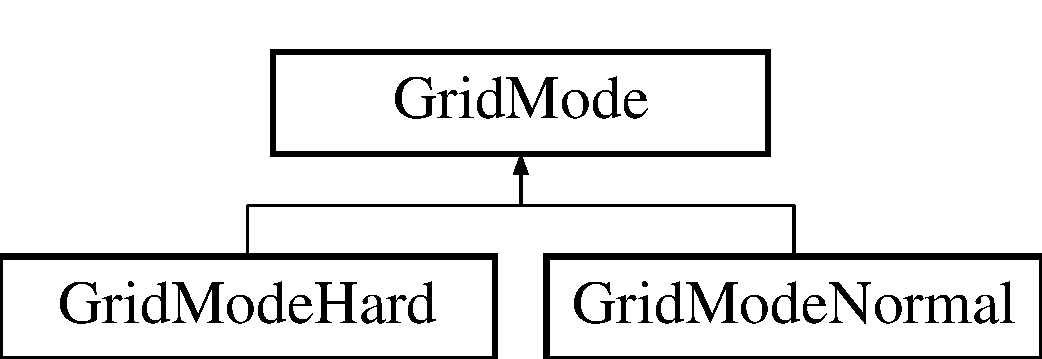
\includegraphics[height=2.000000cm]{classGridMode}
\end{center}
\end{figure}
\subsection*{Public Member Functions}
\begin{DoxyCompactItemize}
\item 
virtual \hyperlink{classGridMode_af8114be34d86c818713ba7105c9f43e9}{$\sim$\-Grid\-Mode} ()
\begin{DoxyCompactList}\small\item\em \char`\"{}\-Constructeur\char`\"{} \end{DoxyCompactList}\item 
virtual bool \hyperlink{classGridMode_a7be800f6198509b3143e221bb3cdde0a}{purge} (\hyperlink{classGrid}{Grid} $\ast$grid)=0
\begin{DoxyCompactList}\small\item\em methode purge \end{DoxyCompactList}\end{DoxyCompactItemize}


\subsection{Detailed Description}
Interface \hyperlink{classGridMode}{Grid\-Mode}. 

\subsection{Constructor \& Destructor Documentation}
\hypertarget{classGridMode_af8114be34d86c818713ba7105c9f43e9}{\index{Grid\-Mode@{Grid\-Mode}!$\sim$\-Grid\-Mode@{$\sim$\-Grid\-Mode}}
\index{$\sim$\-Grid\-Mode@{$\sim$\-Grid\-Mode}!GridMode@{Grid\-Mode}}
\subsubsection[{$\sim$\-Grid\-Mode}]{\setlength{\rightskip}{0pt plus 5cm}virtual Grid\-Mode\-::$\sim$\-Grid\-Mode (
\begin{DoxyParamCaption}
{}
\end{DoxyParamCaption}
)\hspace{0.3cm}{\ttfamily [inline]}, {\ttfamily [virtual]}}}\label{classGridMode_af8114be34d86c818713ba7105c9f43e9}


\char`\"{}\-Constructeur\char`\"{} 

\char`\"{}\-Constructeur\char`\"{} de la classe \hyperlink{classGridMode}{Grid\-Mode} 

\subsection{Member Function Documentation}
\hypertarget{classGridMode_a7be800f6198509b3143e221bb3cdde0a}{\index{Grid\-Mode@{Grid\-Mode}!purge@{purge}}
\index{purge@{purge}!GridMode@{Grid\-Mode}}
\subsubsection[{purge}]{\setlength{\rightskip}{0pt plus 5cm}virtual bool Grid\-Mode\-::purge (
\begin{DoxyParamCaption}
\item[{{\bf Grid} $\ast$}]{grid}
\end{DoxyParamCaption}
)\hspace{0.3cm}{\ttfamily [pure virtual]}}}\label{classGridMode_a7be800f6198509b3143e221bb3cdde0a}


methode purge 


\begin{DoxyParams}{Parameters}
{\em \hyperlink{classGrid}{Grid},pointeur} & sur la grille \\
\hline
\end{DoxyParams}
\begin{DoxyReturn}{Returns}
booléen 
\end{DoxyReturn}


Implemented in \hyperlink{classGridModeHard_a418d223c2d8e6d5af77b0bbf4c10f0e8}{Grid\-Mode\-Hard}, and \hyperlink{classGridModeNormal_a4bcb4bcd60e82c65d2d6c8909b38e5fa}{Grid\-Mode\-Normal}.



The documentation for this class was generated from the following file\-:\begin{DoxyCompactItemize}
\item 
include/Grid\-Mode.\-h\end{DoxyCompactItemize}

\hypertarget{classGridModeHard}{\section{Grid\-Mode\-Hard Class Reference}
\label{classGridModeHard}\index{Grid\-Mode\-Hard@{Grid\-Mode\-Hard}}
}


La classe \hyperlink{classGridModeHard}{Grid\-Mode\-Hard}, implémente la \hyperlink{classGridMode}{Grid\-Mode}.  




{\ttfamily \#include $<$Grid\-Mode\-Hard.\-h$>$}

Inheritance diagram for Grid\-Mode\-Hard\-:\begin{figure}[H]
\begin{center}
\leavevmode
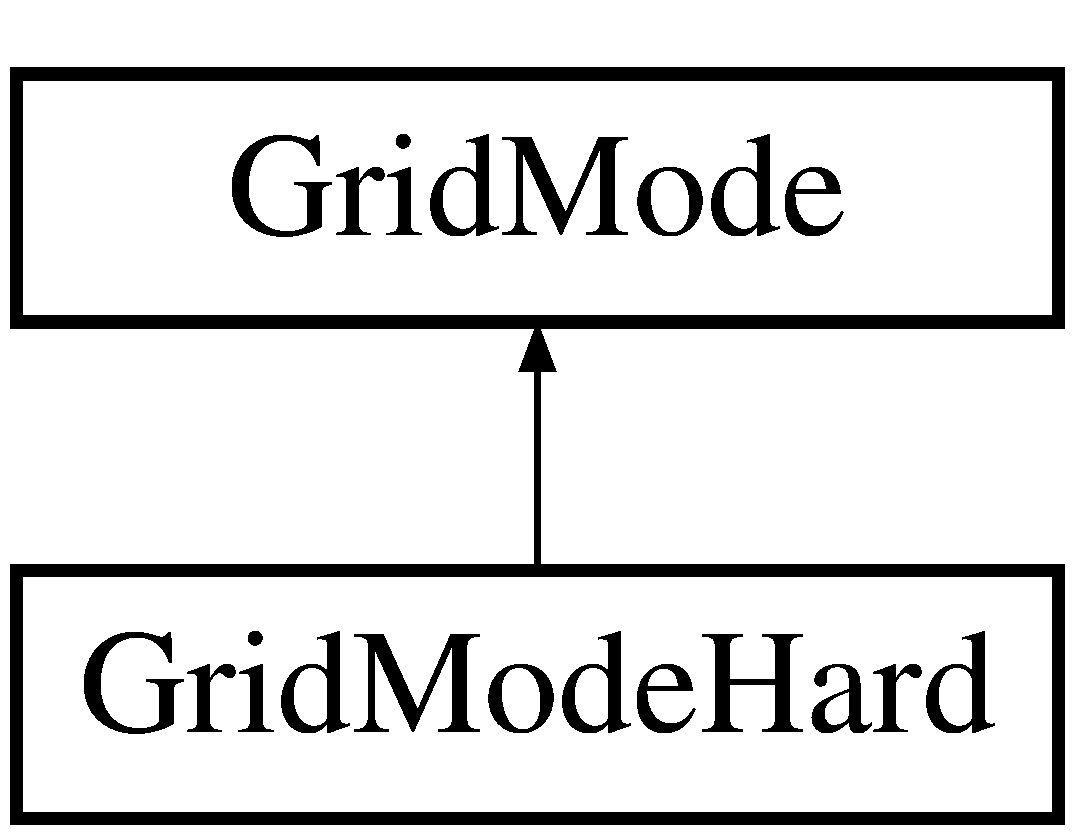
\includegraphics[height=2.000000cm]{classGridModeHard}
\end{center}
\end{figure}
\subsection*{Public Member Functions}
\begin{DoxyCompactItemize}
\item 
\hyperlink{classGridModeHard_a8a91a3b55990849271b8329c6a80b6a1}{Grid\-Mode\-Hard} ()
\begin{DoxyCompactList}\small\item\em Constructeur. \end{DoxyCompactList}\item 
virtual \hyperlink{classGridModeHard_a99545db48decac0df3afcc02e5877b80}{$\sim$\-Grid\-Mode\-Hard} ()
\begin{DoxyCompactList}\small\item\em destructeur \end{DoxyCompactList}\item 
\hypertarget{classGridModeHard_a418d223c2d8e6d5af77b0bbf4c10f0e8}{bool \hyperlink{classGridModeHard_a418d223c2d8e6d5af77b0bbf4c10f0e8}{purge} (\hyperlink{classGrid}{Grid} $\ast$grid)}\label{classGridModeHard_a418d223c2d8e6d5af77b0bbf4c10f0e8}

\begin{DoxyCompactList}\small\item\em methode purge \end{DoxyCompactList}\item 
Vector\-Array2\-I \hyperlink{classGridModeHard_a9293e31f44a67ed00f24f86675368409}{check\-\_\-row} (\hyperlink{classGrid}{Grid} $\ast$grid, int i\-\_\-row)
\begin{DoxyCompactList}\small\item\em methode check\-\_\-row \end{DoxyCompactList}\item 
Vector\-Array2\-I \hyperlink{classGridModeHard_a43cc62651628b27238c653ea244c4129}{check\-\_\-col} (\hyperlink{classGrid}{Grid} $\ast$grid, int i\-\_\-col)
\begin{DoxyCompactList}\small\item\em methode check\-\_\-col \end{DoxyCompactList}\end{DoxyCompactItemize}


\subsection{Detailed Description}
La classe \hyperlink{classGridModeHard}{Grid\-Mode\-Hard}, implémente la \hyperlink{classGridMode}{Grid\-Mode}. 

\subsection{Constructor \& Destructor Documentation}
\hypertarget{classGridModeHard_a8a91a3b55990849271b8329c6a80b6a1}{\index{Grid\-Mode\-Hard@{Grid\-Mode\-Hard}!Grid\-Mode\-Hard@{Grid\-Mode\-Hard}}
\index{Grid\-Mode\-Hard@{Grid\-Mode\-Hard}!GridModeHard@{Grid\-Mode\-Hard}}
\subsubsection[{Grid\-Mode\-Hard}]{\setlength{\rightskip}{0pt plus 5cm}Grid\-Mode\-Hard\-::\-Grid\-Mode\-Hard (
\begin{DoxyParamCaption}
{}
\end{DoxyParamCaption}
)}}\label{classGridModeHard_a8a91a3b55990849271b8329c6a80b6a1}


Constructeur. 

Constructeur de la classe \hyperlink{classGridModeHard}{Grid\-Mode\-Hard} \hypertarget{classGridModeHard_a99545db48decac0df3afcc02e5877b80}{\index{Grid\-Mode\-Hard@{Grid\-Mode\-Hard}!$\sim$\-Grid\-Mode\-Hard@{$\sim$\-Grid\-Mode\-Hard}}
\index{$\sim$\-Grid\-Mode\-Hard@{$\sim$\-Grid\-Mode\-Hard}!GridModeHard@{Grid\-Mode\-Hard}}
\subsubsection[{$\sim$\-Grid\-Mode\-Hard}]{\setlength{\rightskip}{0pt plus 5cm}virtual Grid\-Mode\-Hard\-::$\sim$\-Grid\-Mode\-Hard (
\begin{DoxyParamCaption}
{}
\end{DoxyParamCaption}
)\hspace{0.3cm}{\ttfamily [virtual]}}}\label{classGridModeHard_a99545db48decac0df3afcc02e5877b80}


destructeur 

destructeur de la classe \hyperlink{classGridModeHard}{Grid\-Mode\-Hard} 

\subsection{Member Function Documentation}
\hypertarget{classGridModeHard_a43cc62651628b27238c653ea244c4129}{\index{Grid\-Mode\-Hard@{Grid\-Mode\-Hard}!check\-\_\-col@{check\-\_\-col}}
\index{check\-\_\-col@{check\-\_\-col}!GridModeHard@{Grid\-Mode\-Hard}}
\subsubsection[{check\-\_\-col}]{\setlength{\rightskip}{0pt plus 5cm}Vector\-Array2\-I Grid\-Mode\-Hard\-::check\-\_\-col (
\begin{DoxyParamCaption}
\item[{{\bf Grid} $\ast$}]{grid, }
\item[{int}]{i\-\_\-col}
\end{DoxyParamCaption}
)}}\label{classGridModeHard_a43cc62651628b27238c653ea244c4129}


methode check\-\_\-col 

méthode qui vérifie la colonne i\-\_\-col de la grille, retourne la liste des éléments à retirer 
\begin{DoxyParams}{Parameters}
{\em \hyperlink{classGrid}{Grid},la} & grille sur laquelle vérifier la ligne \\
\hline
{\em Entier,la} & colonne à vérifier \\
\hline
\end{DoxyParams}
\begin{DoxyReturn}{Returns}
Vector\-Array2\-I, la liste des éléments à retirer 
\end{DoxyReturn}
\hypertarget{classGridModeHard_a9293e31f44a67ed00f24f86675368409}{\index{Grid\-Mode\-Hard@{Grid\-Mode\-Hard}!check\-\_\-row@{check\-\_\-row}}
\index{check\-\_\-row@{check\-\_\-row}!GridModeHard@{Grid\-Mode\-Hard}}
\subsubsection[{check\-\_\-row}]{\setlength{\rightskip}{0pt plus 5cm}Vector\-Array2\-I Grid\-Mode\-Hard\-::check\-\_\-row (
\begin{DoxyParamCaption}
\item[{{\bf Grid} $\ast$}]{grid, }
\item[{int}]{i\-\_\-row}
\end{DoxyParamCaption}
)}}\label{classGridModeHard_a9293e31f44a67ed00f24f86675368409}


methode check\-\_\-row 

méthode qui vérifie la ligne i\-\_\-row de la grille, retourne la liste des éléments à retirer 
\begin{DoxyParams}{Parameters}
{\em \hyperlink{classGrid}{Grid},la} & grille sur laquelle vérifier la ligne \\
\hline
{\em Entier,la} & ligne à vérifier \\
\hline
\end{DoxyParams}
\begin{DoxyReturn}{Returns}
Vector\-Array2\-I, la liste des éléments à retirer 
\end{DoxyReturn}


The documentation for this class was generated from the following file\-:\begin{DoxyCompactItemize}
\item 
include/Grid\-Mode\-Hard.\-h\end{DoxyCompactItemize}

\hypertarget{classGridModeNormal}{\section{Grid\-Mode\-Normal Class Reference}
\label{classGridModeNormal}\index{Grid\-Mode\-Normal@{Grid\-Mode\-Normal}}
}


La classe \hyperlink{classGridModeNormal}{Grid\-Mode\-Normal}, implémente la \hyperlink{classGridMode}{Grid\-Mode}.  




{\ttfamily \#include $<$Grid\-Mode\-Normal.\-h$>$}

Inheritance diagram for Grid\-Mode\-Normal\-:\begin{figure}[H]
\begin{center}
\leavevmode
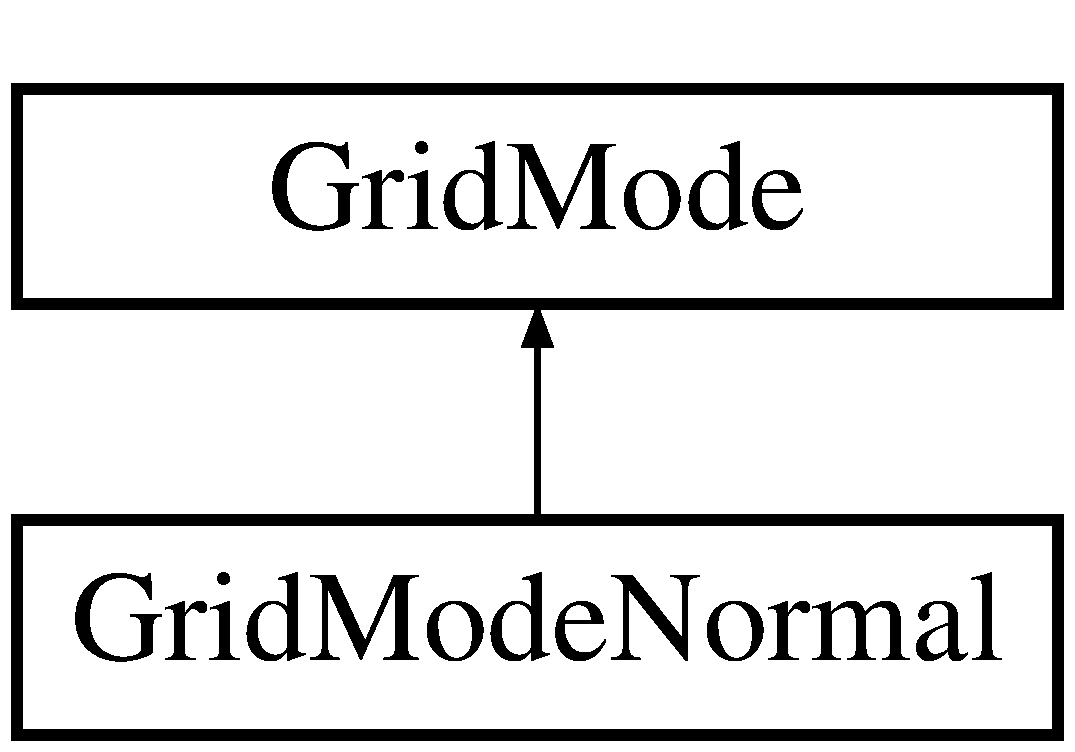
\includegraphics[height=2.000000cm]{classGridModeNormal}
\end{center}
\end{figure}
\subsection*{Public Member Functions}
\begin{DoxyCompactItemize}
\item 
\hyperlink{classGridModeNormal_a1e0d7a4d499cc8bcecb32db771f722c1}{Grid\-Mode\-Normal} ()
\begin{DoxyCompactList}\small\item\em Constructeur. \end{DoxyCompactList}\item 
virtual \hyperlink{classGridModeNormal_a639e48cf51310fa3a39f0ff5a954d5a2}{$\sim$\-Grid\-Mode\-Normal} ()
\begin{DoxyCompactList}\small\item\em destructeur \end{DoxyCompactList}\item 
\hypertarget{classGridModeNormal_a4bcb4bcd60e82c65d2d6c8909b38e5fa}{bool \hyperlink{classGridModeNormal_a4bcb4bcd60e82c65d2d6c8909b38e5fa}{purge} (\hyperlink{classGrid}{Grid} $\ast$grid)}\label{classGridModeNormal_a4bcb4bcd60e82c65d2d6c8909b38e5fa}

\begin{DoxyCompactList}\small\item\em methode purge \end{DoxyCompactList}\item 
Vector\-Array2\-I \hyperlink{classGridModeNormal_a3949d24da71761d187217282f8c1f2e8}{adjacent\-With} (int i, int j, Vector\-Array2\-I $\ast$crossed, \hyperlink{classGrid}{Grid} $\ast$grid)
\begin{DoxyCompactList}\small\item\em methode purge \end{DoxyCompactList}\item 
bool \hyperlink{classGridModeNormal_ab58ed641dd0a89f6eb2976e8e638a8d8}{is\-Crossed} (int i, int j, Vector\-Array2\-I crossed)
\begin{DoxyCompactList}\small\item\em methode is\-Crossed \end{DoxyCompactList}\end{DoxyCompactItemize}


\subsection{Detailed Description}
La classe \hyperlink{classGridModeNormal}{Grid\-Mode\-Normal}, implémente la \hyperlink{classGridMode}{Grid\-Mode}. 

\subsection{Constructor \& Destructor Documentation}
\hypertarget{classGridModeNormal_a1e0d7a4d499cc8bcecb32db771f722c1}{\index{Grid\-Mode\-Normal@{Grid\-Mode\-Normal}!Grid\-Mode\-Normal@{Grid\-Mode\-Normal}}
\index{Grid\-Mode\-Normal@{Grid\-Mode\-Normal}!GridModeNormal@{Grid\-Mode\-Normal}}
\subsubsection[{Grid\-Mode\-Normal}]{\setlength{\rightskip}{0pt plus 5cm}Grid\-Mode\-Normal\-::\-Grid\-Mode\-Normal (
\begin{DoxyParamCaption}
{}
\end{DoxyParamCaption}
)}}\label{classGridModeNormal_a1e0d7a4d499cc8bcecb32db771f722c1}


Constructeur. 

Constructeur de la classe \hyperlink{classGridModeNormal}{Grid\-Mode\-Normal} \hypertarget{classGridModeNormal_a639e48cf51310fa3a39f0ff5a954d5a2}{\index{Grid\-Mode\-Normal@{Grid\-Mode\-Normal}!$\sim$\-Grid\-Mode\-Normal@{$\sim$\-Grid\-Mode\-Normal}}
\index{$\sim$\-Grid\-Mode\-Normal@{$\sim$\-Grid\-Mode\-Normal}!GridModeNormal@{Grid\-Mode\-Normal}}
\subsubsection[{$\sim$\-Grid\-Mode\-Normal}]{\setlength{\rightskip}{0pt plus 5cm}virtual Grid\-Mode\-Normal\-::$\sim$\-Grid\-Mode\-Normal (
\begin{DoxyParamCaption}
{}
\end{DoxyParamCaption}
)\hspace{0.3cm}{\ttfamily [virtual]}}}\label{classGridModeNormal_a639e48cf51310fa3a39f0ff5a954d5a2}


destructeur 

destructeur de la classe \hyperlink{classGridModeNormal}{Grid\-Mode\-Normal} 

\subsection{Member Function Documentation}
\hypertarget{classGridModeNormal_a3949d24da71761d187217282f8c1f2e8}{\index{Grid\-Mode\-Normal@{Grid\-Mode\-Normal}!adjacent\-With@{adjacent\-With}}
\index{adjacent\-With@{adjacent\-With}!GridModeNormal@{Grid\-Mode\-Normal}}
\subsubsection[{adjacent\-With}]{\setlength{\rightskip}{0pt plus 5cm}Vector\-Array2\-I Grid\-Mode\-Normal\-::adjacent\-With (
\begin{DoxyParamCaption}
\item[{int}]{i, }
\item[{int}]{j, }
\item[{Vector\-Array2\-I $\ast$}]{crossed, }
\item[{{\bf Grid} $\ast$}]{grid}
\end{DoxyParamCaption}
)}}\label{classGridModeNormal_a3949d24da71761d187217282f8c1f2e8}


methode purge 

méthode qui vérifie si l'élément (i, j) est adjacent avec d'autres éléments de même type que lui 
\begin{DoxyParams}{Parameters}
{\em Entier,position} & i de l'élément \\
\hline
{\em Entier,position} & j de l'élément \\
\hline
{\em Vector\-Array2\-I,pointeur} & vers liste des éléments avec les adjacents D\-E\-J\-A analysés \\
\hline
{\em \hyperlink{classGrid}{Grid},la} & grille \\
\hline
\end{DoxyParams}
\begin{DoxyReturn}{Returns}
Vector\-Array2\-I , la liste d'éléments 
\end{DoxyReturn}
\hypertarget{classGridModeNormal_ab58ed641dd0a89f6eb2976e8e638a8d8}{\index{Grid\-Mode\-Normal@{Grid\-Mode\-Normal}!is\-Crossed@{is\-Crossed}}
\index{is\-Crossed@{is\-Crossed}!GridModeNormal@{Grid\-Mode\-Normal}}
\subsubsection[{is\-Crossed}]{\setlength{\rightskip}{0pt plus 5cm}bool Grid\-Mode\-Normal\-::is\-Crossed (
\begin{DoxyParamCaption}
\item[{int}]{i, }
\item[{int}]{j, }
\item[{Vector\-Array2\-I}]{crossed}
\end{DoxyParamCaption}
)}}\label{classGridModeNormal_ab58ed641dd0a89f6eb2976e8e638a8d8}


methode is\-Crossed 


\begin{DoxyParams}{Parameters}
{\em Entier,position} & i de l'élément\\
\hline
{\em Vector\-Array2\-I,pointeur} & vers liste des éléments avec les adjacents D\-E\-J\-A analysés \\
\hline
\end{DoxyParams}


The documentation for this class was generated from the following file\-:\begin{DoxyCompactItemize}
\item 
include/Grid\-Mode\-Normal.\-h\end{DoxyCompactItemize}

\hypertarget{classMenuScreen}{\section{Menu\-Screen Class Reference}
\label{classMenuScreen}\index{Menu\-Screen@{Menu\-Screen}}
}


La classe \hyperlink{classMenuScreen}{Menu\-Screen}, Implémente l'interface \hyperlink{classScreen}{Screen}.  




{\ttfamily \#include $<$Menu\-Screen.\-h$>$}

Inheritance diagram for Menu\-Screen\-:\begin{figure}[H]
\begin{center}
\leavevmode
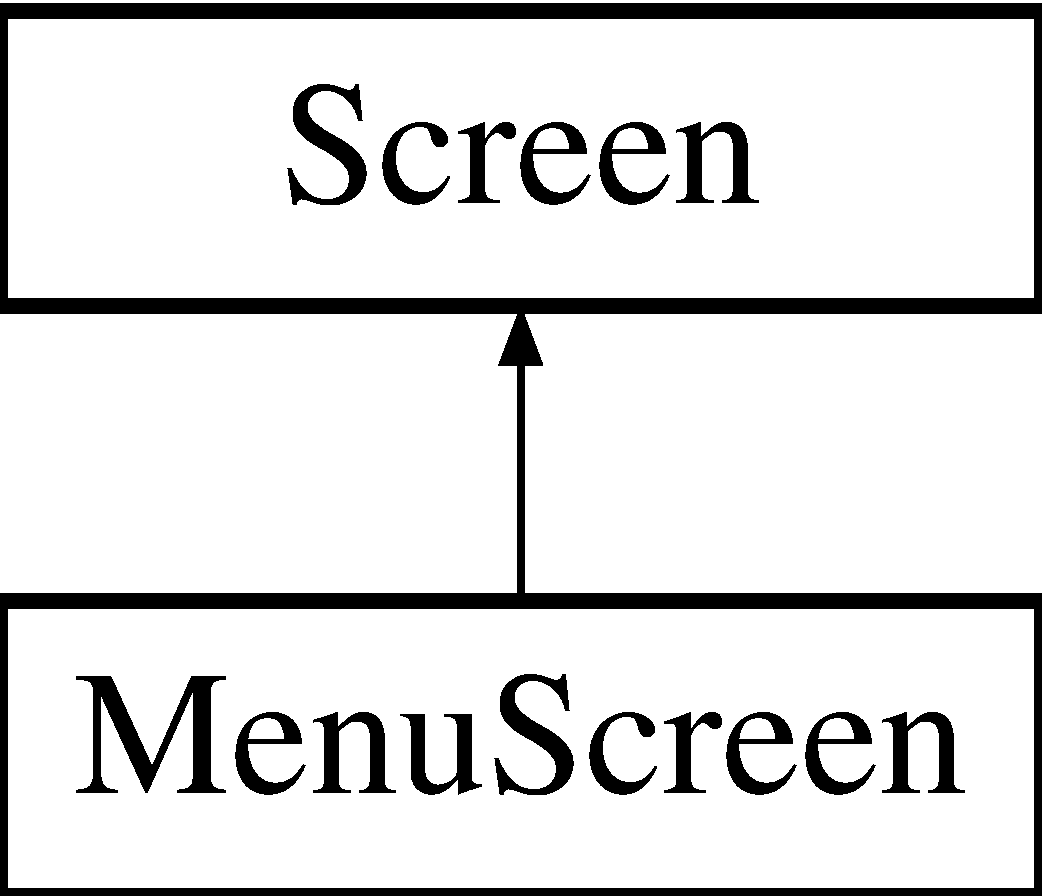
\includegraphics[height=2.000000cm]{classMenuScreen}
\end{center}
\end{figure}
\subsection*{Public Member Functions}
\begin{DoxyCompactItemize}
\item 
\hyperlink{classMenuScreen_a1b1207941e5331afa594befc3fd5d857}{Menu\-Screen} (\hyperlink{classEngine}{Engine} $\ast$engine)
\begin{DoxyCompactList}\small\item\em Constructeur. \end{DoxyCompactList}\item 
virtual \hyperlink{classMenuScreen_aa5d98169f4d2e3ef2e6520a6a5bbc47c}{$\sim$\-Menu\-Screen} ()
\begin{DoxyCompactList}\small\item\em Destructeur. \end{DoxyCompactList}\item 
void \hyperlink{classMenuScreen_a6ff381327f56f7e40ae481f28b241bd2}{show} (S\-D\-L\-\_\-\-Surface $\ast$screen)
\begin{DoxyCompactList}\small\item\em methode show \end{DoxyCompactList}\item 
void \hyperlink{classMenuScreen_ac26706ac22c9db9d980c9fc63315d843}{render} (S\-D\-L\-\_\-\-Surface $\ast$screen)
\begin{DoxyCompactList}\small\item\em methode render \end{DoxyCompactList}\item 
void \hyperlink{classMenuScreen_a92fe1ecb63138057739cd6325179ef9a}{resize} (S\-D\-L\-\_\-\-Surface $\ast$screen)
\begin{DoxyCompactList}\small\item\em methode resize \end{DoxyCompactList}\item 
void \hyperlink{classMenuScreen_a6e1f118966c89b894c02ad7181e1c994}{hide} (S\-D\-L\-\_\-\-Surface $\ast$screen)
\begin{DoxyCompactList}\small\item\em methode hide \end{DoxyCompactList}\item 
void \hyperlink{classMenuScreen_afbffa22948c7e335e5db27233bc661b9}{event} (S\-D\-L\-\_\-\-Event $\ast$event, bool $\ast$loop)
\begin{DoxyCompactList}\small\item\em methode event \end{DoxyCompactList}\item 
void \hyperlink{classMenuScreen_a7ac89f1f67d52d3659901e0bce76054c}{mouse\-Click} (int x, int y)
\begin{DoxyCompactList}\small\item\em methode mouse\-Click \end{DoxyCompactList}\item 
\hypertarget{classMenuScreen_a372890c5387b89ea63c146cc0b05b02c}{\hyperlink{classEngine}{Engine} $\ast$ \hyperlink{classMenuScreen_a372890c5387b89ea63c146cc0b05b02c}{get\-Engine} ()}\label{classMenuScreen_a372890c5387b89ea63c146cc0b05b02c}

\begin{DoxyCompactList}\small\item\em methode qui retourne le pointeur sur le moteur du jeu \end{DoxyCompactList}\end{DoxyCompactItemize}


\subsection{Detailed Description}
La classe \hyperlink{classMenuScreen}{Menu\-Screen}, Implémente l'interface \hyperlink{classScreen}{Screen}. 

\subsection{Constructor \& Destructor Documentation}
\hypertarget{classMenuScreen_a1b1207941e5331afa594befc3fd5d857}{\index{Menu\-Screen@{Menu\-Screen}!Menu\-Screen@{Menu\-Screen}}
\index{Menu\-Screen@{Menu\-Screen}!MenuScreen@{Menu\-Screen}}
\subsubsection[{Menu\-Screen}]{\setlength{\rightskip}{0pt plus 5cm}Menu\-Screen\-::\-Menu\-Screen (
\begin{DoxyParamCaption}
\item[{{\bf Engine} $\ast$}]{engine}
\end{DoxyParamCaption}
)}}\label{classMenuScreen_a1b1207941e5331afa594befc3fd5d857}


Constructeur. 

Constructeur de la classe \hyperlink{classMenuScreen}{Menu\-Screen} 
\begin{DoxyParams}{Parameters}
{\em \hyperlink{classEngine}{Engine},le} & moteur de jeu \\
\hline
\end{DoxyParams}
\hypertarget{classMenuScreen_aa5d98169f4d2e3ef2e6520a6a5bbc47c}{\index{Menu\-Screen@{Menu\-Screen}!$\sim$\-Menu\-Screen@{$\sim$\-Menu\-Screen}}
\index{$\sim$\-Menu\-Screen@{$\sim$\-Menu\-Screen}!MenuScreen@{Menu\-Screen}}
\subsubsection[{$\sim$\-Menu\-Screen}]{\setlength{\rightskip}{0pt plus 5cm}virtual Menu\-Screen\-::$\sim$\-Menu\-Screen (
\begin{DoxyParamCaption}
{}
\end{DoxyParamCaption}
)\hspace{0.3cm}{\ttfamily [virtual]}}}\label{classMenuScreen_aa5d98169f4d2e3ef2e6520a6a5bbc47c}


Destructeur. 

Destructeur de la classe \hyperlink{classMenuScreen}{Menu\-Screen} 

\subsection{Member Function Documentation}
\hypertarget{classMenuScreen_afbffa22948c7e335e5db27233bc661b9}{\index{Menu\-Screen@{Menu\-Screen}!event@{event}}
\index{event@{event}!MenuScreen@{Menu\-Screen}}
\subsubsection[{event}]{\setlength{\rightskip}{0pt plus 5cm}void Menu\-Screen\-::event (
\begin{DoxyParamCaption}
\item[{S\-D\-L\-\_\-\-Event $\ast$}]{event, }
\item[{bool $\ast$}]{loop}
\end{DoxyParamCaption}
)\hspace{0.3cm}{\ttfamily [virtual]}}}\label{classMenuScreen_afbffa22948c7e335e5db27233bc661b9}


methode event 

methode qui gère l'ensemble des événements liés à l'écran


\begin{DoxyParams}{Parameters}
{\em S\-D\-L\-\_\-\-Event,l'évenement} & sdl \\
\hline
{\em booléen,la} & boucle \\
\hline
\end{DoxyParams}


Implements \hyperlink{classScreen_a072825d7520cba6d89beaa4e173a6b81}{Screen}.

\hypertarget{classMenuScreen_a6e1f118966c89b894c02ad7181e1c994}{\index{Menu\-Screen@{Menu\-Screen}!hide@{hide}}
\index{hide@{hide}!MenuScreen@{Menu\-Screen}}
\subsubsection[{hide}]{\setlength{\rightskip}{0pt plus 5cm}void Menu\-Screen\-::hide (
\begin{DoxyParamCaption}
\item[{S\-D\-L\-\_\-\-Surface $\ast$}]{screen}
\end{DoxyParamCaption}
)\hspace{0.3cm}{\ttfamily [virtual]}}}\label{classMenuScreen_a6e1f118966c89b894c02ad7181e1c994}


methode hide 

methode qui \char`\"{}cache\char`\"{} l'écran


\begin{DoxyParams}{Parameters}
{\em S\-Dl\-\_\-\-Surface} & \\
\hline
\end{DoxyParams}


Implements \hyperlink{classScreen_a04c451ca44c902190d9f0c20b5585a69}{Screen}.

\hypertarget{classMenuScreen_a7ac89f1f67d52d3659901e0bce76054c}{\index{Menu\-Screen@{Menu\-Screen}!mouse\-Click@{mouse\-Click}}
\index{mouse\-Click@{mouse\-Click}!MenuScreen@{Menu\-Screen}}
\subsubsection[{mouse\-Click}]{\setlength{\rightskip}{0pt plus 5cm}void Menu\-Screen\-::mouse\-Click (
\begin{DoxyParamCaption}
\item[{int}]{x, }
\item[{int}]{y}
\end{DoxyParamCaption}
)\hspace{0.3cm}{\ttfamily [virtual]}}}\label{classMenuScreen_a7ac89f1f67d52d3659901e0bce76054c}


methode mouse\-Click 

methode qui permet la gestion du clique sur l'écran


\begin{DoxyParams}{Parameters}
{\em entier,l'abscisse} & \\
\hline
{\em entier,l'ordonnée} & \\
\hline
\end{DoxyParams}


Implements \hyperlink{classScreen_a03916a6d13cebf61e730086ef7650d1e}{Screen}.

\hypertarget{classMenuScreen_ac26706ac22c9db9d980c9fc63315d843}{\index{Menu\-Screen@{Menu\-Screen}!render@{render}}
\index{render@{render}!MenuScreen@{Menu\-Screen}}
\subsubsection[{render}]{\setlength{\rightskip}{0pt plus 5cm}void Menu\-Screen\-::render (
\begin{DoxyParamCaption}
\item[{S\-D\-L\-\_\-\-Surface $\ast$}]{screen}
\end{DoxyParamCaption}
)\hspace{0.3cm}{\ttfamily [virtual]}}}\label{classMenuScreen_ac26706ac22c9db9d980c9fc63315d843}


methode render 

methode qui gère l'affichage de l'écran


\begin{DoxyParams}{Parameters}
{\em S\-Dl\-\_\-\-Surface,l'écran} & \\
\hline
\end{DoxyParams}


Implements \hyperlink{classScreen_a54b82c1f1ba74e82451dde46481c27f1}{Screen}.

\hypertarget{classMenuScreen_a92fe1ecb63138057739cd6325179ef9a}{\index{Menu\-Screen@{Menu\-Screen}!resize@{resize}}
\index{resize@{resize}!MenuScreen@{Menu\-Screen}}
\subsubsection[{resize}]{\setlength{\rightskip}{0pt plus 5cm}void Menu\-Screen\-::resize (
\begin{DoxyParamCaption}
\item[{S\-D\-L\-\_\-\-Surface $\ast$}]{screen}
\end{DoxyParamCaption}
)\hspace{0.3cm}{\ttfamily [virtual]}}}\label{classMenuScreen_a92fe1ecb63138057739cd6325179ef9a}


methode resize 

methode qui permet de redimensionner la taille de la fenêtre


\begin{DoxyParams}{Parameters}
{\em S\-Dl\-\_\-\-Surface,l'écran} & a redimensionner \\
\hline
\end{DoxyParams}


Implements \hyperlink{classScreen_aae326b09506351ccf22c34a22b8eae40}{Screen}.

\hypertarget{classMenuScreen_a6ff381327f56f7e40ae481f28b241bd2}{\index{Menu\-Screen@{Menu\-Screen}!show@{show}}
\index{show@{show}!MenuScreen@{Menu\-Screen}}
\subsubsection[{show}]{\setlength{\rightskip}{0pt plus 5cm}void Menu\-Screen\-::show (
\begin{DoxyParamCaption}
\item[{S\-D\-L\-\_\-\-Surface $\ast$}]{screen}
\end{DoxyParamCaption}
)\hspace{0.3cm}{\ttfamily [virtual]}}}\label{classMenuScreen_a6ff381327f56f7e40ae481f28b241bd2}


methode show 

methode permettant d'afficher l'écran ( appeler une fois )


\begin{DoxyParams}{Parameters}
{\em S\-Dl\-\_\-\-Surface,l'écran} & \\
\hline
\end{DoxyParams}


Implements \hyperlink{classScreen_ae875c48e44e67e4a1e5211337d67577f}{Screen}.



The documentation for this class was generated from the following file\-:\begin{DoxyCompactItemize}
\item 
include/Menu\-Screen.\-h\end{DoxyCompactItemize}

\hypertarget{classPlayer}{\section{Player Class Reference}
\label{classPlayer}\index{Player@{Player}}
}


La classe \hyperlink{classPlayer}{Player}.  




{\ttfamily \#include $<$Player.\-h$>$}

\subsection*{Public Member Functions}
\begin{DoxyCompactItemize}
\item 
\hyperlink{classPlayer_affe0cc3cb714f6deb4e62f0c0d3f1fd8}{Player} ()
\begin{DoxyCompactList}\small\item\em Constructeur. \end{DoxyCompactList}\item 
\hyperlink{classPlayer_a0e93e5237600a8160ee5632f41068252}{Player} (string name, int money, vector$<$ int $>$ highscore)
\begin{DoxyCompactList}\small\item\em Surchage du Constructeur. \end{DoxyCompactList}\item 
virtual \hyperlink{classPlayer_a8981c201ffb2270c0b6dbd467b627376}{$\sim$\-Player} ()
\begin{DoxyCompactList}\small\item\em Destructeur. \end{DoxyCompactList}\item 
\hypertarget{classPlayer_af9a6045fa96f736664c4eab4caa5e8e5}{string {\bfseries get\-Name} ()}\label{classPlayer_af9a6045fa96f736664c4eab4caa5e8e5}

\item 
\hypertarget{classPlayer_ac45154df7c4eb2d1d58255c3ff1c55dd}{int {\bfseries get\-Money} ()}\label{classPlayer_ac45154df7c4eb2d1d58255c3ff1c55dd}

\item 
\hypertarget{classPlayer_a25096c68b44eae33a189bdf65383afff}{vector$<$ int $>$ {\bfseries get\-Highscore} ()}\label{classPlayer_a25096c68b44eae33a189bdf65383afff}

\item 
\hypertarget{classPlayer_a6e78f6a0e2e73323bf200a9e1c2e0ac6}{void {\bfseries set\-Money} (int money)}\label{classPlayer_a6e78f6a0e2e73323bf200a9e1c2e0ac6}

\item 
\hypertarget{classPlayer_af1a4192c97234896cc60cecd817ff2b0}{void {\bfseries set\-Highscore} (vector$<$ int $>$ highscore)}\label{classPlayer_af1a4192c97234896cc60cecd817ff2b0}

\item 
\hypertarget{classPlayer_aa9728db5b22d438505b4694c5ea03f75}{void {\bfseries set\-Name} (string name)}\label{classPlayer_aa9728db5b22d438505b4694c5ea03f75}

\end{DoxyCompactItemize}


\subsection{Detailed Description}
La classe \hyperlink{classPlayer}{Player}. 

\subsection{Constructor \& Destructor Documentation}
\hypertarget{classPlayer_affe0cc3cb714f6deb4e62f0c0d3f1fd8}{\index{Player@{Player}!Player@{Player}}
\index{Player@{Player}!Player@{Player}}
\subsubsection[{Player}]{\setlength{\rightskip}{0pt plus 5cm}Player\-::\-Player (
\begin{DoxyParamCaption}
{}
\end{DoxyParamCaption}
)}}\label{classPlayer_affe0cc3cb714f6deb4e62f0c0d3f1fd8}


Constructeur. 

Constructeur de la classe \hyperlink{classPlayer}{Player} \hypertarget{classPlayer_a0e93e5237600a8160ee5632f41068252}{\index{Player@{Player}!Player@{Player}}
\index{Player@{Player}!Player@{Player}}
\subsubsection[{Player}]{\setlength{\rightskip}{0pt plus 5cm}Player\-::\-Player (
\begin{DoxyParamCaption}
\item[{string}]{name, }
\item[{int}]{money, }
\item[{vector$<$ int $>$}]{highscore}
\end{DoxyParamCaption}
)}}\label{classPlayer_a0e93e5237600a8160ee5632f41068252}


Surchage du Constructeur. 

Surchage du Constructeur de la classe \hyperlink{classPlayer}{Player} 
\begin{DoxyParams}{Parameters}
{\em string,le} & nom du joueur \\
\hline
{\em Entier,money} & l'argent du joueur \\
\hline
{\em vector$<$int$>$,liste} & des score du joueur \\
\hline
\end{DoxyParams}
\hypertarget{classPlayer_a8981c201ffb2270c0b6dbd467b627376}{\index{Player@{Player}!$\sim$\-Player@{$\sim$\-Player}}
\index{$\sim$\-Player@{$\sim$\-Player}!Player@{Player}}
\subsubsection[{$\sim$\-Player}]{\setlength{\rightskip}{0pt plus 5cm}virtual Player\-::$\sim$\-Player (
\begin{DoxyParamCaption}
{}
\end{DoxyParamCaption}
)\hspace{0.3cm}{\ttfamily [virtual]}}}\label{classPlayer_a8981c201ffb2270c0b6dbd467b627376}


Destructeur. 

Destructeur de la classe \hyperlink{classPlayer}{Player} 

The documentation for this class was generated from the following file\-:\begin{DoxyCompactItemize}
\item 
include/Player.\-h\end{DoxyCompactItemize}

\hypertarget{classPointBonusElement}{\section{Point\-Bonus\-Element Class Reference}
\label{classPointBonusElement}\index{Point\-Bonus\-Element@{Point\-Bonus\-Element}}
}


La classe \hyperlink{classPointBonusElement}{Point\-Bonus\-Element}, hérite de \hyperlink{classBaseElement}{Base\-Element}.  




{\ttfamily \#include $<$Point\-Bonus\-Element.\-h$>$}

Inheritance diagram for Point\-Bonus\-Element\-:\begin{figure}[H]
\begin{center}
\leavevmode
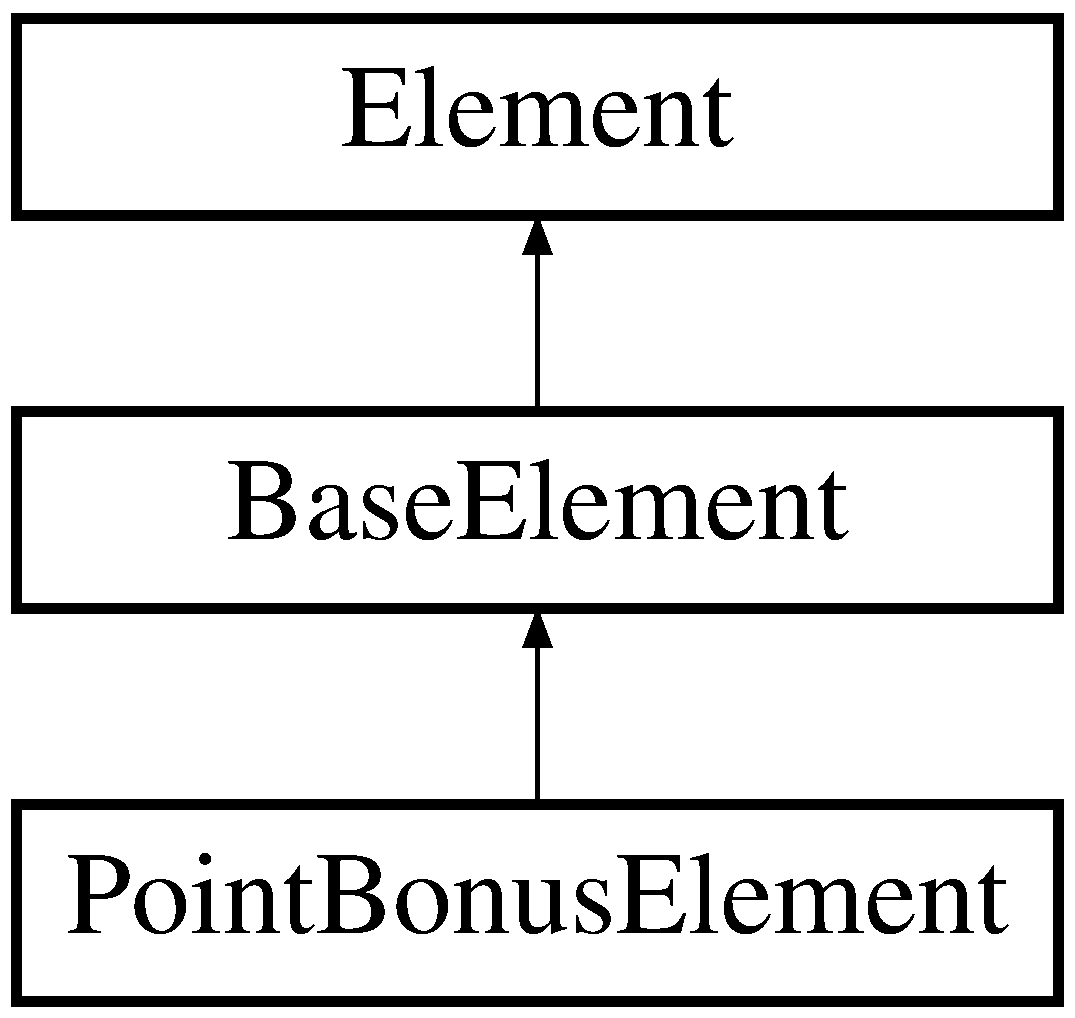
\includegraphics[height=3.000000cm]{classPointBonusElement}
\end{center}
\end{figure}
\subsection*{Public Member Functions}
\begin{DoxyCompactItemize}
\item 
\hyperlink{classPointBonusElement_a79141a25bc092d979a06e0ef0b618cd2}{Point\-Bonus\-Element} (\hyperlink{classElement}{Element} el)
\begin{DoxyCompactList}\small\item\em Constructeur. \end{DoxyCompactList}\item 
virtual \hyperlink{classPointBonusElement_a6e0edec449969d256c70c2cd6e238ab0}{$\sim$\-Point\-Bonus\-Element} ()
\begin{DoxyCompactList}\small\item\em Destructeur. \end{DoxyCompactList}\item 
int \hyperlink{classPointBonusElement_a5766494f3f66abcda8bd125779b4082a}{get\-Value} ()
\begin{DoxyCompactList}\small\item\em Accesseur. \end{DoxyCompactList}\item 
int \hyperlink{classPointBonusElement_ad8cea3552abfcbb657b29575798b45cb}{get\-Money} ()
\begin{DoxyCompactList}\small\item\em Accesseur. \end{DoxyCompactList}\end{DoxyCompactItemize}
\subsection*{Additional Inherited Members}


\subsection{Detailed Description}
La classe \hyperlink{classPointBonusElement}{Point\-Bonus\-Element}, hérite de \hyperlink{classBaseElement}{Base\-Element}. 

\subsection{Constructor \& Destructor Documentation}
\hypertarget{classPointBonusElement_a79141a25bc092d979a06e0ef0b618cd2}{\index{Point\-Bonus\-Element@{Point\-Bonus\-Element}!Point\-Bonus\-Element@{Point\-Bonus\-Element}}
\index{Point\-Bonus\-Element@{Point\-Bonus\-Element}!PointBonusElement@{Point\-Bonus\-Element}}
\subsubsection[{Point\-Bonus\-Element}]{\setlength{\rightskip}{0pt plus 5cm}Point\-Bonus\-Element\-::\-Point\-Bonus\-Element (
\begin{DoxyParamCaption}
\item[{{\bf Element}}]{el}
\end{DoxyParamCaption}
)}}\label{classPointBonusElement_a79141a25bc092d979a06e0ef0b618cd2}


Constructeur. 

Constructeur de la classe \hyperlink{classPointBonusElement}{Point\-Bonus\-Element} 
\begin{DoxyParams}{Parameters}
{\em \hyperlink{classElement}{Element},l'élément} & à décoré \\
\hline
\end{DoxyParams}
\hypertarget{classPointBonusElement_a6e0edec449969d256c70c2cd6e238ab0}{\index{Point\-Bonus\-Element@{Point\-Bonus\-Element}!$\sim$\-Point\-Bonus\-Element@{$\sim$\-Point\-Bonus\-Element}}
\index{$\sim$\-Point\-Bonus\-Element@{$\sim$\-Point\-Bonus\-Element}!PointBonusElement@{Point\-Bonus\-Element}}
\subsubsection[{$\sim$\-Point\-Bonus\-Element}]{\setlength{\rightskip}{0pt plus 5cm}virtual Point\-Bonus\-Element\-::$\sim$\-Point\-Bonus\-Element (
\begin{DoxyParamCaption}
{}
\end{DoxyParamCaption}
)\hspace{0.3cm}{\ttfamily [virtual]}}}\label{classPointBonusElement_a6e0edec449969d256c70c2cd6e238ab0}


Destructeur. 

Destructeur de la classe \hyperlink{classPointBonusElement}{Point\-Bonus\-Element} 

\subsection{Member Function Documentation}
\hypertarget{classPointBonusElement_ad8cea3552abfcbb657b29575798b45cb}{\index{Point\-Bonus\-Element@{Point\-Bonus\-Element}!get\-Money@{get\-Money}}
\index{get\-Money@{get\-Money}!PointBonusElement@{Point\-Bonus\-Element}}
\subsubsection[{get\-Money}]{\setlength{\rightskip}{0pt plus 5cm}int Point\-Bonus\-Element\-::get\-Money (
\begin{DoxyParamCaption}
{}
\end{DoxyParamCaption}
)}}\label{classPointBonusElement_ad8cea3552abfcbb657b29575798b45cb}


Accesseur. 

accesseur de l'attribut money de l'élément \hypertarget{classPointBonusElement_a5766494f3f66abcda8bd125779b4082a}{\index{Point\-Bonus\-Element@{Point\-Bonus\-Element}!get\-Value@{get\-Value}}
\index{get\-Value@{get\-Value}!PointBonusElement@{Point\-Bonus\-Element}}
\subsubsection[{get\-Value}]{\setlength{\rightskip}{0pt plus 5cm}int Point\-Bonus\-Element\-::get\-Value (
\begin{DoxyParamCaption}
{}
\end{DoxyParamCaption}
)}}\label{classPointBonusElement_a5766494f3f66abcda8bd125779b4082a}


Accesseur. 

accesseur de l'attribut valeur de l'élément 

The documentation for this class was generated from the following file\-:\begin{DoxyCompactItemize}
\item 
include/Point\-Bonus\-Element.\-h\end{DoxyCompactItemize}

\hypertarget{classScreen}{\section{Screen Class Reference}
\label{classScreen}\index{Screen@{Screen}}
}


Interface \hyperlink{classScreen}{Screen}.  




{\ttfamily \#include $<$Screen.\-h$>$}

Inheritance diagram for Screen\-:\begin{figure}[H]
\begin{center}
\leavevmode
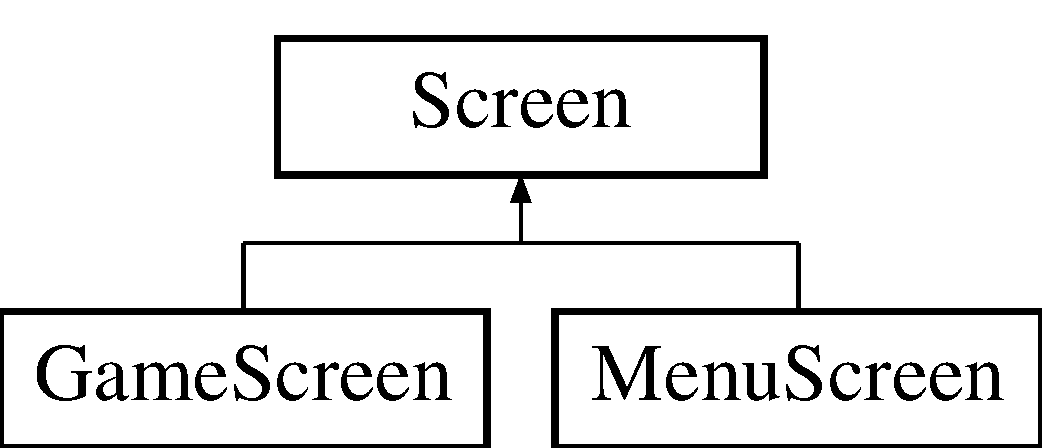
\includegraphics[height=2.000000cm]{classScreen}
\end{center}
\end{figure}
\subsection*{Public Member Functions}
\begin{DoxyCompactItemize}
\item 
virtual void \hyperlink{classScreen_ae875c48e44e67e4a1e5211337d67577f}{show} (S\-D\-L\-\_\-\-Surface $\ast$screen)=0
\begin{DoxyCompactList}\small\item\em methode show \end{DoxyCompactList}\item 
virtual void \hyperlink{classScreen_a54b82c1f1ba74e82451dde46481c27f1}{render} (S\-D\-L\-\_\-\-Surface $\ast$screen)=0
\begin{DoxyCompactList}\small\item\em methode render \end{DoxyCompactList}\item 
virtual void \hyperlink{classScreen_aae326b09506351ccf22c34a22b8eae40}{resize} (S\-D\-L\-\_\-\-Surface $\ast$screen)=0
\begin{DoxyCompactList}\small\item\em methode resize \end{DoxyCompactList}\item 
virtual void \hyperlink{classScreen_a04c451ca44c902190d9f0c20b5585a69}{hide} (S\-D\-L\-\_\-\-Surface $\ast$screen)=0
\begin{DoxyCompactList}\small\item\em methode hide \end{DoxyCompactList}\item 
virtual void \hyperlink{classScreen_a072825d7520cba6d89beaa4e173a6b81}{event} (S\-D\-L\-\_\-\-Event $\ast$event, bool $\ast$loop)=0
\begin{DoxyCompactList}\small\item\em methode event \end{DoxyCompactList}\item 
virtual void \hyperlink{classScreen_a03916a6d13cebf61e730086ef7650d1e}{mouse\-Click} (int x, int y)=0
\begin{DoxyCompactList}\small\item\em methode mouse\-Click \end{DoxyCompactList}\end{DoxyCompactItemize}


\subsection{Detailed Description}
Interface \hyperlink{classScreen}{Screen}. 

\subsection{Member Function Documentation}
\hypertarget{classScreen_a072825d7520cba6d89beaa4e173a6b81}{\index{Screen@{Screen}!event@{event}}
\index{event@{event}!Screen@{Screen}}
\subsubsection[{event}]{\setlength{\rightskip}{0pt plus 5cm}virtual void Screen\-::event (
\begin{DoxyParamCaption}
\item[{S\-D\-L\-\_\-\-Event $\ast$}]{event, }
\item[{bool $\ast$}]{loop}
\end{DoxyParamCaption}
)\hspace{0.3cm}{\ttfamily [pure virtual]}}}\label{classScreen_a072825d7520cba6d89beaa4e173a6b81}


methode event 

methode qui gère l'ensemble des événements liés à l'écran


\begin{DoxyParams}{Parameters}
{\em S\-D\-L\-\_\-\-Event,l'évenement} & sdl \\
\hline
{\em booléen,la} & boucle \\
\hline
\end{DoxyParams}


Implemented in \hyperlink{classGameScreen_a542fcc8ed203427ea442bb2f52406a91}{Game\-Screen}, and \hyperlink{classMenuScreen_afbffa22948c7e335e5db27233bc661b9}{Menu\-Screen}.

\hypertarget{classScreen_a04c451ca44c902190d9f0c20b5585a69}{\index{Screen@{Screen}!hide@{hide}}
\index{hide@{hide}!Screen@{Screen}}
\subsubsection[{hide}]{\setlength{\rightskip}{0pt plus 5cm}virtual void Screen\-::hide (
\begin{DoxyParamCaption}
\item[{S\-D\-L\-\_\-\-Surface $\ast$}]{screen}
\end{DoxyParamCaption}
)\hspace{0.3cm}{\ttfamily [pure virtual]}}}\label{classScreen_a04c451ca44c902190d9f0c20b5585a69}


methode hide 

methode qui \char`\"{}cache\char`\"{} l'écran


\begin{DoxyParams}{Parameters}
{\em S\-Dl\-\_\-\-Surface} & \\
\hline
\end{DoxyParams}


Implemented in \hyperlink{classGameScreen_ac818a2dc8c094fc2bb23ceb0a0a53cf3}{Game\-Screen}, and \hyperlink{classMenuScreen_a6e1f118966c89b894c02ad7181e1c994}{Menu\-Screen}.

\hypertarget{classScreen_a03916a6d13cebf61e730086ef7650d1e}{\index{Screen@{Screen}!mouse\-Click@{mouse\-Click}}
\index{mouse\-Click@{mouse\-Click}!Screen@{Screen}}
\subsubsection[{mouse\-Click}]{\setlength{\rightskip}{0pt plus 5cm}virtual void Screen\-::mouse\-Click (
\begin{DoxyParamCaption}
\item[{int}]{x, }
\item[{int}]{y}
\end{DoxyParamCaption}
)\hspace{0.3cm}{\ttfamily [pure virtual]}}}\label{classScreen_a03916a6d13cebf61e730086ef7650d1e}


methode mouse\-Click 

methode qui permet la gestion du clique sur l'écran


\begin{DoxyParams}{Parameters}
{\em entier,l'abscisse} & \\
\hline
{\em entier,l'ordonnée} & \\
\hline
\end{DoxyParams}


Implemented in \hyperlink{classGameScreen_a46f96d4b6a0bbd02e83ce25318912c47}{Game\-Screen}, and \hyperlink{classMenuScreen_a7ac89f1f67d52d3659901e0bce76054c}{Menu\-Screen}.

\hypertarget{classScreen_a54b82c1f1ba74e82451dde46481c27f1}{\index{Screen@{Screen}!render@{render}}
\index{render@{render}!Screen@{Screen}}
\subsubsection[{render}]{\setlength{\rightskip}{0pt plus 5cm}virtual void Screen\-::render (
\begin{DoxyParamCaption}
\item[{S\-D\-L\-\_\-\-Surface $\ast$}]{screen}
\end{DoxyParamCaption}
)\hspace{0.3cm}{\ttfamily [pure virtual]}}}\label{classScreen_a54b82c1f1ba74e82451dde46481c27f1}


methode render 

methode qui gère l'affichage de l'écran


\begin{DoxyParams}{Parameters}
{\em S\-Dl\-\_\-\-Surface,l'écran} & \\
\hline
\end{DoxyParams}


Implemented in \hyperlink{classGameScreen_a8f4d95f64f07e01b4ebe35b31b39acb7}{Game\-Screen}, and \hyperlink{classMenuScreen_ac26706ac22c9db9d980c9fc63315d843}{Menu\-Screen}.

\hypertarget{classScreen_aae326b09506351ccf22c34a22b8eae40}{\index{Screen@{Screen}!resize@{resize}}
\index{resize@{resize}!Screen@{Screen}}
\subsubsection[{resize}]{\setlength{\rightskip}{0pt plus 5cm}virtual void Screen\-::resize (
\begin{DoxyParamCaption}
\item[{S\-D\-L\-\_\-\-Surface $\ast$}]{screen}
\end{DoxyParamCaption}
)\hspace{0.3cm}{\ttfamily [pure virtual]}}}\label{classScreen_aae326b09506351ccf22c34a22b8eae40}


methode resize 

methode qui permet de redimensionner la taille de la fenêtre


\begin{DoxyParams}{Parameters}
{\em S\-Dl\-\_\-\-Surface,l'écran} & a redimensionner \\
\hline
\end{DoxyParams}


Implemented in \hyperlink{classGameScreen_a0b4bad004b986f9aeed9b8f69606c11b}{Game\-Screen}, and \hyperlink{classMenuScreen_a92fe1ecb63138057739cd6325179ef9a}{Menu\-Screen}.

\hypertarget{classScreen_ae875c48e44e67e4a1e5211337d67577f}{\index{Screen@{Screen}!show@{show}}
\index{show@{show}!Screen@{Screen}}
\subsubsection[{show}]{\setlength{\rightskip}{0pt plus 5cm}virtual void Screen\-::show (
\begin{DoxyParamCaption}
\item[{S\-D\-L\-\_\-\-Surface $\ast$}]{screen}
\end{DoxyParamCaption}
)\hspace{0.3cm}{\ttfamily [pure virtual]}}}\label{classScreen_ae875c48e44e67e4a1e5211337d67577f}


methode show 

methode permettant d'afficher l'écran ( appeler une fois )


\begin{DoxyParams}{Parameters}
{\em S\-Dl\-\_\-\-Surface,l'écran} & \\
\hline
\end{DoxyParams}


Implemented in \hyperlink{classGameScreen_a43a2a1a9c28f8e2892ae3d91e1dcfa1f}{Game\-Screen}, and \hyperlink{classMenuScreen_a6ff381327f56f7e40ae481f28b241bd2}{Menu\-Screen}.



The documentation for this class was generated from the following file\-:\begin{DoxyCompactItemize}
\item 
include/Screen.\-h\end{DoxyCompactItemize}

%--- End generated contents ---

% Index
\newpage
\phantomsection
\addcontentsline{toc}{part}{Index}
\printindex

\end{document}
